\documentclass[1p]{elsarticle_modified}
%\bibliographystyle{elsarticle-num}

%\usepackage[colorlinks]{hyperref}
%\usepackage{abbrmath_seonhwa} %\Abb, \Ascr, \Acal ,\Abf, \Afrak
\usepackage{amsfonts}
\usepackage{amssymb}
\usepackage{amsmath}
\usepackage{amsthm}
\usepackage{scalefnt}
\usepackage{amsbsy}
\usepackage{kotex}
\usepackage{caption}
\usepackage{subfig}
\usepackage{color}
\usepackage{graphicx}
\usepackage{xcolor} %% white, black, red, green, blue, cyan, magenta, yellow
\usepackage{float}
\usepackage{setspace}
\usepackage{hyperref}

\usepackage{tikz}
\usetikzlibrary{arrows}

\usepackage{multirow}
\usepackage{array} % fixed length table
\usepackage{hhline}

%%%%%%%%%%%%%%%%%%%%%
\makeatletter
\renewcommand*\env@matrix[1][\arraystretch]{%
	\edef\arraystretch{#1}%
	\hskip -\arraycolsep
	\let\@ifnextchar\new@ifnextchar
	\array{*\c@MaxMatrixCols c}}
\makeatother %https://tex.stackexchange.com/questions/14071/how-can-i-increase-the-line-spacing-in-a-matrix
%%%%%%%%%%%%%%%

\usepackage[normalem]{ulem}

\newcommand{\msout}[1]{\ifmmode\text{\sout{\ensuremath{#1}}}\else\sout{#1}\fi}
%SOURCE: \msout is \stkout macro in https://tex.stackexchange.com/questions/20609/strikeout-in-math-mode

\newcommand{\cancel}[1]{
	\ifmmode
	{\color{red}\msout{#1}}
	\else
	{\color{red}\sout{#1}}
	\fi
}

\newcommand{\add}[1]{
	{\color{blue}\uwave{#1}}
}

\newcommand{\replace}[2]{
	\ifmmode
	{\color{red}\msout{#1}}{\color{blue}\uwave{#2}}
	\else
	{\color{red}\sout{#1}}{\color{blue}\uwave{#2}}
	\fi
}

\newcommand{\Sol}{\mathcal{S}} %segment
\newcommand{\D}{D} %diagram
\newcommand{\A}{\mathcal{A}} %arc


%%%%%%%%%%%%%%%%%%%%%%%%%%%%%5 test

\def\sl{\operatorname{\textup{SL}}(2,\Cbb)}
\def\psl{\operatorname{\textup{PSL}}(2,\Cbb)}
\def\quan{\mkern 1mu \triangleright \mkern 1mu}

\theoremstyle{definition}
\newtheorem{thm}{Theorem}[section]
\newtheorem{prop}[thm]{Proposition}
\newtheorem{lem}[thm]{Lemma}
\newtheorem{ques}[thm]{Question}
\newtheorem{cor}[thm]{Corollary}
\newtheorem{defn}[thm]{Definition}
\newtheorem{exam}[thm]{Example}
\newtheorem{rmk}[thm]{Remark}
\newtheorem{alg}[thm]{Algorithm}

\newcommand{\I}{\sqrt{-1}}
\begin{document}

%\begin{frontmatter}
%
%\title{Boundary parabolic representations of knots up to 8 crossings}
%
%%% Group authors per affiliation:
%\author{Yunhi Cho} 
%\address{Department of Mathematics, University of Seoul, Seoul, Korea}
%\ead{yhcho@uos.ac.kr}
%
%
%\author{Seonhwa Kim} %\fnref{s_kim}}
%\address{Center for Geometry and Physics, Institute for Basic Science, Pohang, 37673, Korea}
%\ead{ryeona17@ibs.re.kr}
%
%\author{Hyuk Kim}
%\address{Department of Mathematical Sciences, Seoul National University, Seoul 08826, Korea}
%\ead{hyukkim@snu.ac.kr}
%
%\author{Seokbeom Yoon}
%\address{Department of Mathematical Sciences, Seoul National University, Seoul, 08826,  Korea}
%\ead{sbyoon15@snu.ac.kr}
%
%\begin{abstract}
%We find all boundary parabolic representation of knots up to 8 crossings.
%
%\end{abstract}
%\begin{keyword}
%    \MSC[2010] 57M25 
%\end{keyword}
%
%\end{frontmatter}

%\linenumbers
%\tableofcontents
%
\newcommand\colored[1]{\textcolor{white}{\rule[-0.35ex]{0.8em}{1.4ex}}\kern-0.8em\color{red} #1}%
%\newcommand\colored[1]{\textcolor{white}{ #1}\kern-2.17ex	\textcolor{white}{ #1}\kern-1.81ex	\textcolor{white}{ #1}\kern-2.15ex\color{red}#1	}

{\Large $\underline{12a_{0546}~(K12a_{0546})}$}

\setlength{\tabcolsep}{10pt}
\renewcommand{\arraystretch}{1.6}
\vspace{1cm}\begin{tabular}{m{100pt}>{\centering\arraybackslash}m{274pt}}
\multirow{5}{120pt}{
	\centering
	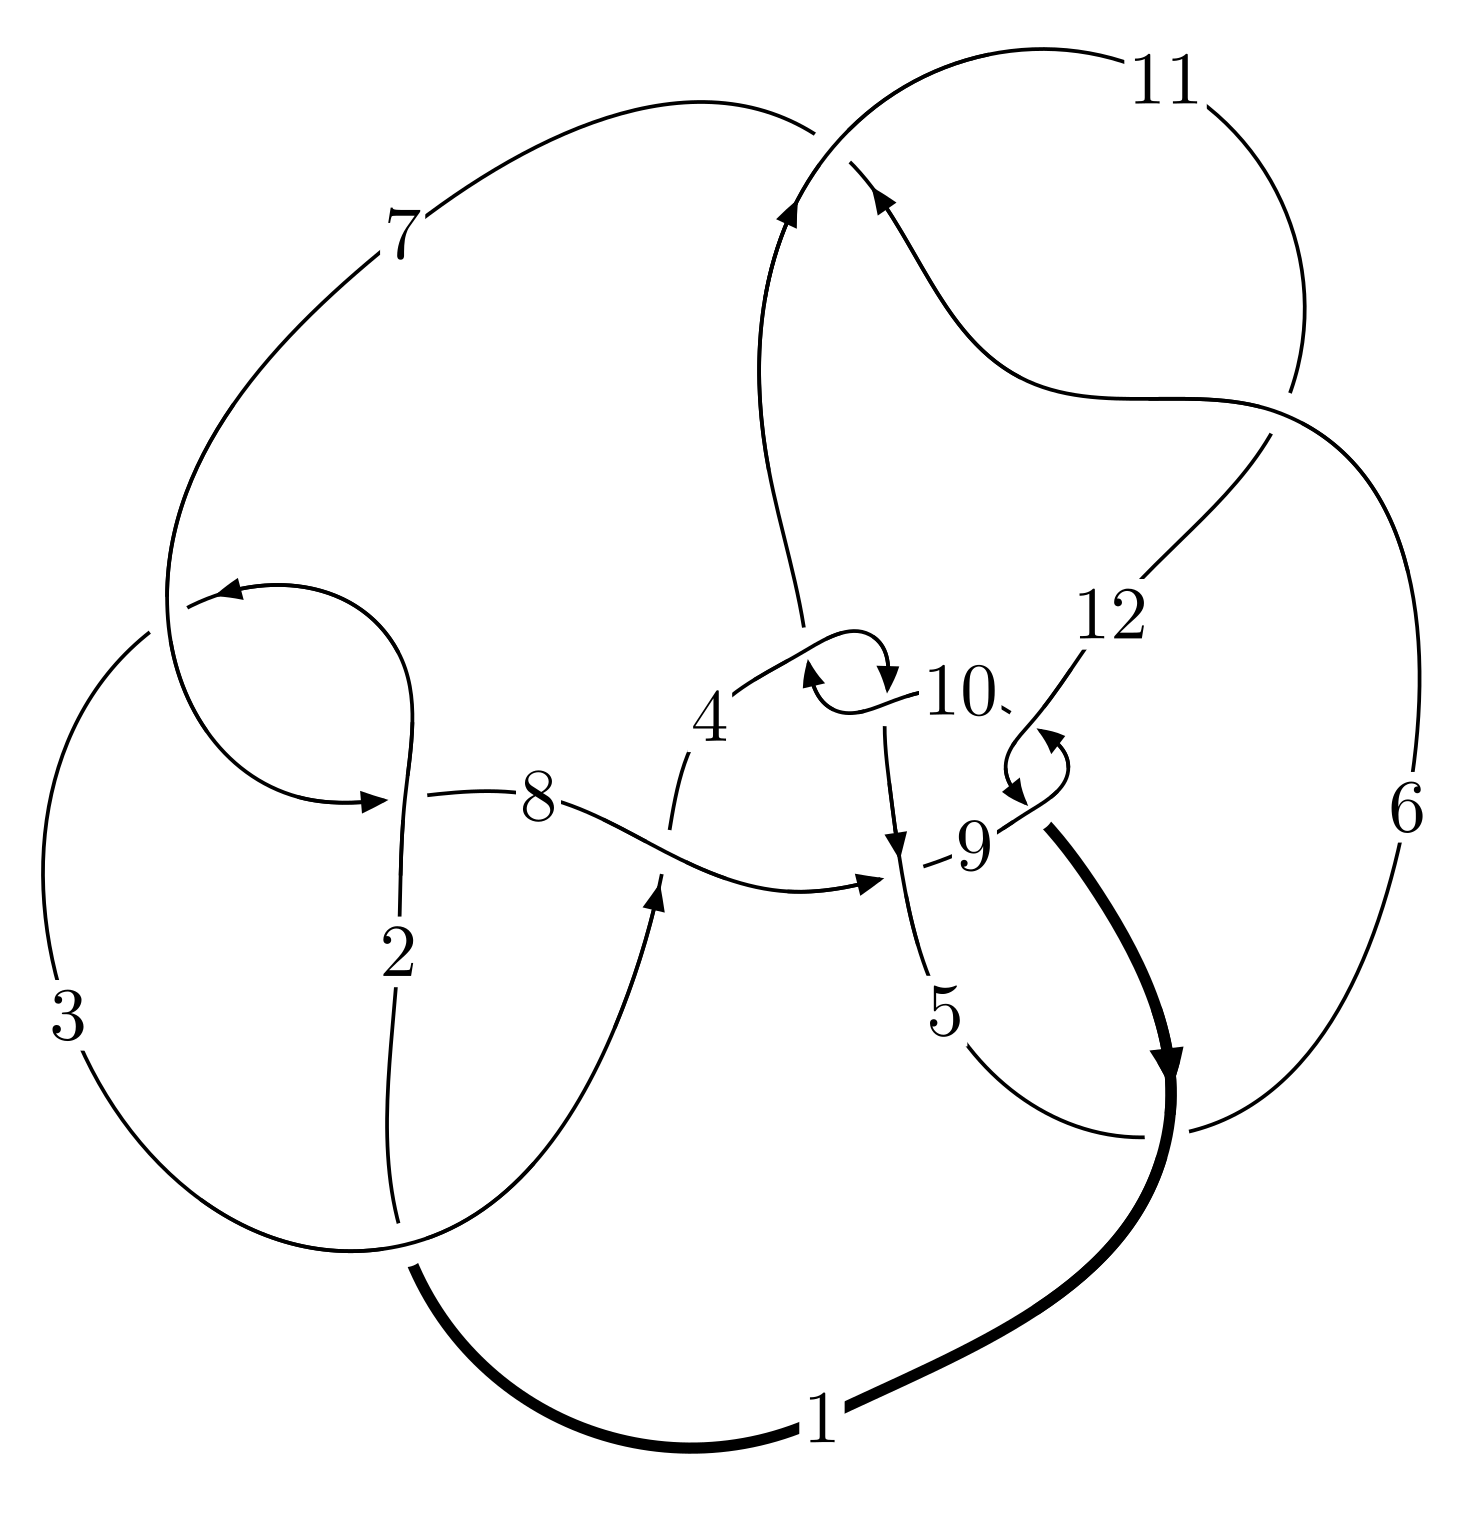
\includegraphics[width=112pt]{../../../GIT/diagram.site/Diagrams/png/1347_12a_0546.png}\\
\ \ \ A knot diagram\footnotemark}&
\allowdisplaybreaks
\textbf{Linearized knot diagam} \\
\cline{2-2}
 &
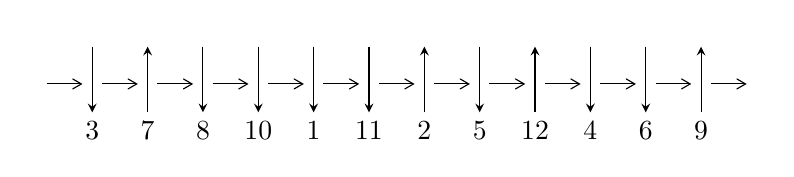
\begin{tikzpicture}[x=20pt, y=17pt]
	% nodes
	\node (C0) at (0, 0) {};
	\node (C1) at (1, 0) {};
	\node (C1U) at (1, +1) {};
	\node (C1D) at (1, -1) {3};

	\node (C2) at (2, 0) {};
	\node (C2U) at (2, +1) {};
	\node (C2D) at (2, -1) {7};

	\node (C3) at (3, 0) {};
	\node (C3U) at (3, +1) {};
	\node (C3D) at (3, -1) {8};

	\node (C4) at (4, 0) {};
	\node (C4U) at (4, +1) {};
	\node (C4D) at (4, -1) {10};

	\node (C5) at (5, 0) {};
	\node (C5U) at (5, +1) {};
	\node (C5D) at (5, -1) {1};

	\node (C6) at (6, 0) {};
	\node (C6U) at (6, +1) {};
	\node (C6D) at (6, -1) {11};

	\node (C7) at (7, 0) {};
	\node (C7U) at (7, +1) {};
	\node (C7D) at (7, -1) {2};

	\node (C8) at (8, 0) {};
	\node (C8U) at (8, +1) {};
	\node (C8D) at (8, -1) {5};

	\node (C9) at (9, 0) {};
	\node (C9U) at (9, +1) {};
	\node (C9D) at (9, -1) {12};

	\node (C10) at (10, 0) {};
	\node (C10U) at (10, +1) {};
	\node (C10D) at (10, -1) {4};

	\node (C11) at (11, 0) {};
	\node (C11U) at (11, +1) {};
	\node (C11D) at (11, -1) {6};

	\node (C12) at (12, 0) {};
	\node (C12U) at (12, +1) {};
	\node (C12D) at (12, -1) {9};
	\node (C13) at (13, 0) {};

	% arrows
	\draw[->,>={angle 60}]
	(C0) edge (C1) (C1) edge (C2) (C2) edge (C3) (C3) edge (C4) (C4) edge (C5) (C5) edge (C6) (C6) edge (C7) (C7) edge (C8) (C8) edge (C9) (C9) edge (C10) (C10) edge (C11) (C11) edge (C12) (C12) edge (C13) ;	\draw[->,>=stealth]
	(C1U) edge (C1D) (C2D) edge (C2U) (C3U) edge (C3D) (C4U) edge (C4D) (C5U) edge (C5D) (C6U) edge (C6D) (C7D) edge (C7U) (C8U) edge (C8D) (C9D) edge (C9U) (C10U) edge (C10D) (C11U) edge (C11D) (C12D) edge (C12U) ;
	\end{tikzpicture} \\
\hhline{~~} \\& 
\textbf{Solving Sequence} \\ \cline{2-2} 
 &
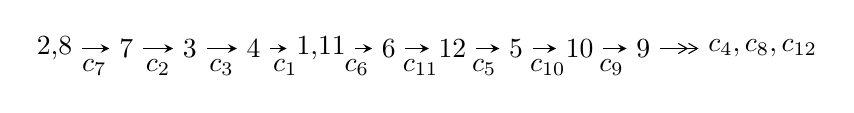
\begin{tikzpicture}[x=23pt, y=7pt]
	% node
	\node (A0) at (-1/8, 0) {2,8};
	\node (A1) at (1, 0) {7};
	\node (A2) at (2, 0) {3};
	\node (A3) at (3, 0) {4};
	\node (A4) at (65/16, 0) {1,11};
	\node (A5) at (41/8, 0) {6};
	\node (A6) at (49/8, 0) {12};
	\node (A7) at (57/8, 0) {5};
	\node (A8) at (65/8, 0) {10};
	\node (A9) at (73/8, 0) {9};
	\node (C1) at (1/2, -1) {$c_{7}$};
	\node (C2) at (3/2, -1) {$c_{2}$};
	\node (C3) at (5/2, -1) {$c_{3}$};
	\node (C4) at (7/2, -1) {$c_{1}$};
	\node (C5) at (37/8, -1) {$c_{6}$};
	\node (C6) at (45/8, -1) {$c_{11}$};
	\node (C7) at (53/8, -1) {$c_{5}$};
	\node (C8) at (61/8, -1) {$c_{10}$};
	\node (C9) at (69/8, -1) {$c_{9}$};
	\node (A10) at (11, 0) {$c_{4},c_{8},c_{12}$};

	% edge
	\draw[->,>=stealth]	
	(A0) edge (A1) (A1) edge (A2) (A2) edge (A3) (A3) edge (A4) (A4) edge (A5) (A5) edge (A6) (A6) edge (A7) (A7) edge (A8) (A8) edge (A9) ;
	\draw[->>,>={angle 60}]	
	(A9) edge (A10);
\end{tikzpicture} \\ 

\end{tabular} \\

\footnotetext{
The image of knot diagram is generated by the software ``\textbf{Draw programme}" developed by Andrew Bartholomew(\url{http://www.layer8.co.uk/maths/draw/index.htm\#Running-draw}), where we modified some parts for our purpose(\url{https://github.com/CATsTAILs/LinksPainter}).
}\phantom \\ \newline 
\centering \textbf{Ideals for irreducible components\footnotemark of $X_{\text{par}}$} 
 
\begin{align*}
I^u_{1}&=\langle 
-177 u^{48}-2295 u^{47}+\cdots+16 b-22288,\;-1039 u^{48}-10379 u^{47}+\cdots+32 a-6640,\\
\phantom{I^u_{1}}&\phantom{= \langle  }u^{49}+11 u^{48}+\cdots+336 u+32\rangle \\
I^u_{2}&=\langle 
-3.75564\times10^{34} a^{9} u^{3}+9.36038\times10^{34} a^{8} u^{3}+\cdots+3.47750\times10^{34} a-1.15768\times10^{36},\\
\phantom{I^u_{2}}&\phantom{= \langle  }- a^9 u^3+8 a^8 u^3+\cdots-140 a+56,\;u^4+u^2+u+1\rangle \\
I^u_{3}&=\langle 
4 u^{33}- u^{32}+\cdots+b-3,\;- u^{33}+5 u^{32}+\cdots+a+6,\;u^{34}+9 u^{32}+\cdots+5 u^2+1\rangle \\
I^u_{4}&=\langle 
-1.40412\times10^{42} a^{9} u^{5}-1.78290\times10^{42} a^{8} u^{5}+\cdots-6.44973\times10^{41} a-1.75326\times10^{42},\\
\phantom{I^u_{4}}&\phantom{= \langle  }- a^8 u^5-5 a^7 u^5+\cdots+43 a+33,\;u^6- u^5+2 u^4-2 u^3+2 u^2-2 u+1\rangle \\
\\
\end{align*}
\raggedright * 4 irreducible components of $\dim_{\mathbb{C}}=0$, with total 183 representations.\\
\footnotetext{All coefficients of polynomials are rational numbers. But the coefficients are sometimes approximated in decimal forms when there is not enough margin.}
\newpage
\renewcommand{\arraystretch}{1}
\centering \section*{I. $I^u_{1}= \langle -177 u^{48}-2295 u^{47}+\cdots+16 b-22288,\;-1039 u^{48}-10379 u^{47}+\cdots+32 a-6640,\;u^{49}+11 u^{48}+\cdots+336 u+32 \rangle$}
\flushleft \textbf{(i) Arc colorings}\\
\begin{tabular}{m{7pt} m{180pt} m{7pt} m{180pt} }
\flushright $a_{2}=$&$\begin{pmatrix}0\\u\end{pmatrix}$ \\
\flushright $a_{8}=$&$\begin{pmatrix}1\\0\end{pmatrix}$ \\
\flushright $a_{7}=$&$\begin{pmatrix}1\\u^2\end{pmatrix}$ \\
\flushright $a_{3}=$&$\begin{pmatrix}u\\u^3+u\end{pmatrix}$ \\
\flushright $a_{4}=$&$\begin{pmatrix}- u^3\\u^3+u\end{pmatrix}$ \\
\flushright $a_{1}=$&$\begin{pmatrix}u^3\\u^5+u^3+u\end{pmatrix}$ \\
\flushright $a_{11}=$&$\begin{pmatrix}\frac{1039}{32} u^{48}+\frac{10379}{32} u^{47}+\cdots+2331 u+\frac{415}{2}\\\frac{177}{16} u^{48}+\frac{2295}{16} u^{47}+\cdots+13026 u+1393\end{pmatrix}$ \\
\flushright $a_{6}=$&$\begin{pmatrix}\frac{1}{2} u^{48}-8 u^{47}+\cdots-2888 u-\frac{607}{2}\\15 u^{48}+\frac{327}{2} u^{47}+\cdots+\frac{10033}{2} u+496\end{pmatrix}$ \\
\flushright $a_{12}=$&$\begin{pmatrix}\frac{523}{16} u^{48}+293 u^{47}+\cdots-6815 u-776\\\frac{143}{16} u^{48}+\frac{2251}{16} u^{47}+\cdots+13224 u+1390\end{pmatrix}$ \\
\flushright $a_{5}=$&$\begin{pmatrix}-15 u^{48}-\frac{311}{2} u^{47}+\cdots-2400 u-\frac{447}{2}\\\frac{15}{2} u^{48}+\frac{143}{2} u^{47}+\cdots+\frac{1425}{2} u+80\end{pmatrix}$ \\
\flushright $a_{10}=$&$\begin{pmatrix}-\frac{209}{32} u^{48}-\frac{1493}{32} u^{47}+\cdots+6055 u+\frac{1359}{2}\\\frac{185}{16} u^{48}+\frac{1691}{16} u^{47}+\cdots+1056 u+103\end{pmatrix}$ \\
\flushright $a_{9}=$&$\begin{pmatrix}\frac{21}{2} u^{48}+136 u^{47}+\cdots+\frac{27905}{4} u+705\\-\frac{13}{4} u^{48}-\frac{69}{2} u^{47}+\cdots+1840 u+224\end{pmatrix}$\\&\end{tabular}
\flushleft \textbf{(ii) Obstruction class $= -1$}\\~\\
\flushleft \textbf{(iii) Cusp Shapes $= \frac{13}{2} u^{48}+136 u^{47}+\cdots+19132 u+2014$}\\~\\
\newpage\renewcommand{\arraystretch}{1}
\flushleft \textbf{(iv) u-Polynomials at the component}\newline \\
\begin{tabular}{m{50pt}|m{274pt}}
Crossings & \hspace{64pt}u-Polynomials at each crossing \\
\hline $$\begin{aligned}c_{1}\end{aligned}$$&$\begin{aligned}
&u^{49}+23 u^{48}+\cdots-2304 u-1024
\end{aligned}$\\
\hline $$\begin{aligned}c_{2},c_{7}\end{aligned}$$&$\begin{aligned}
&u^{49}+11 u^{48}+\cdots+336 u+32
\end{aligned}$\\
\hline $$\begin{aligned}c_{3}\end{aligned}$$&$\begin{aligned}
&u^{49}-11 u^{48}+\cdots-1796480 u+194816
\end{aligned}$\\
\hline $$\begin{aligned}c_{4},c_{6},c_{10}\\c_{11}\end{aligned}$$&$\begin{aligned}
&u^{49}+15 u^{47}+\cdots+3 u+1
\end{aligned}$\\
\hline $$\begin{aligned}c_{5},c_{8}\end{aligned}$$&$\begin{aligned}
&u^{49}-13 u^{47}+\cdots+45 u^2+1
\end{aligned}$\\
\hline $$\begin{aligned}c_{9},c_{12}\end{aligned}$$&$\begin{aligned}
&u^{49}+24 u^{48}+\cdots+20992 u+1024
\end{aligned}$\\
\hline
\end{tabular}\\~\\
\newpage\renewcommand{\arraystretch}{1}
\flushleft \textbf{(v) Riley Polynomials at the component}\newline \\
\begin{tabular}{m{50pt}|m{274pt}}
Crossings & \hspace{64pt}Riley Polynomials at each crossing \\
\hline $$\begin{aligned}c_{1}\end{aligned}$$&$\begin{aligned}
&y^{49}+7 y^{48}+\cdots+3342336 y-1048576
\end{aligned}$\\
\hline $$\begin{aligned}c_{2},c_{7}\end{aligned}$$&$\begin{aligned}
&y^{49}+23 y^{48}+\cdots-2304 y-1024
\end{aligned}$\\
\hline $$\begin{aligned}c_{3}\end{aligned}$$&$\begin{aligned}
&y^{49}-9 y^{48}+\cdots+105434251264 y-37953273856
\end{aligned}$\\
\hline $$\begin{aligned}c_{4},c_{6},c_{10}\\c_{11}\end{aligned}$$&$\begin{aligned}
&y^{49}+30 y^{48}+\cdots-7 y-1
\end{aligned}$\\
\hline $$\begin{aligned}c_{5},c_{8}\end{aligned}$$&$\begin{aligned}
&y^{49}-26 y^{48}+\cdots-90 y-1
\end{aligned}$\\
\hline $$\begin{aligned}c_{9},c_{12}\end{aligned}$$&$\begin{aligned}
&y^{49}+18 y^{48}+\cdots-13893632 y-1048576
\end{aligned}$\\
\hline
\end{tabular}\\~\\
\newpage\flushleft \textbf{(vi) Complex Volumes and Cusp Shapes}
$$\begin{array}{c|c|c}  
\text{Solutions to }I^u_{1}& \I (\text{vol} + \sqrt{-1}CS) & \text{Cusp shape}\\
 \hline 
\begin{aligned}
u &= \phantom{-}0.478052 + 0.856443 I \\
a &= \phantom{-}0.326341 - 0.492210 I \\
b &= -0.305506 + 0.147125 I\end{aligned}
 & -1.49827 + 2.65503 I & \phantom{-0.000000 } 0 \\ \hline\begin{aligned}
u &= \phantom{-}0.478052 - 0.856443 I \\
a &= \phantom{-}0.326341 + 0.492210 I \\
b &= -0.305506 - 0.147125 I\end{aligned}
 & -1.49827 - 2.65503 I & \phantom{-0.000000 } 0 \\ \hline\begin{aligned}
u &= \phantom{-}0.766749 + 0.715877 I \\
a &= \phantom{-}0.739711 + 0.674856 I \\
b &= -0.247125 - 0.492473 I\end{aligned}
 & \phantom{-}5.20437 + 10.91700 I & \phantom{-0.000000 } 0 \\ \hline\begin{aligned}
u &= \phantom{-}0.766749 - 0.715877 I \\
a &= \phantom{-}0.739711 - 0.674856 I \\
b &= -0.247125 + 0.492473 I\end{aligned}
 & \phantom{-}5.20437 - 10.91700 I & \phantom{-0.000000 } 0 \\ \hline\begin{aligned}
u &= -0.873499 + 0.354678 I \\
a &= -0.494292 - 0.464853 I \\
b &= -1.10940 + 1.28651 I\end{aligned}
 & \phantom{-}6.00554 + 7.82565 I & \phantom{-0.000000 } 0 \\ \hline\begin{aligned}
u &= -0.873499 - 0.354678 I \\
a &= -0.494292 + 0.464853 I \\
b &= -1.10940 - 1.28651 I\end{aligned}
 & \phantom{-}6.00554 - 7.82565 I & \phantom{-0.000000 } 0 \\ \hline\begin{aligned}
u &= -0.928111 + 0.072870 I \\
a &= \phantom{-}0.0795687 - 0.0803024 I \\
b &= -0.092121 - 1.024010 I\end{aligned}
 & -0.88139 - 3.32643 I & \phantom{-0.000000 } 0 \\ \hline\begin{aligned}
u &= -0.928111 - 0.072870 I \\
a &= \phantom{-}0.0795687 + 0.0803024 I \\
b &= -0.092121 + 1.024010 I\end{aligned}
 & -0.88139 + 3.32643 I & \phantom{-0.000000 } 0 \\ \hline\begin{aligned}
u &= -0.854709 + 0.330936 I \\
a &= \phantom{-}0.589192 + 0.476228 I \\
b &= \phantom{-}1.27262 - 1.43921 I\end{aligned}
 & \phantom{-}2.9680 + 14.0850 I & \phantom{-0.000000 } 0 \\ \hline\begin{aligned}
u &= -0.854709 - 0.330936 I \\
a &= \phantom{-}0.589192 - 0.476228 I \\
b &= \phantom{-}1.27262 + 1.43921 I\end{aligned}
 & \phantom{-}2.9680 - 14.0850 I & \phantom{-0.000000 } 0\\
 \hline 
 \end{array}$$\newpage$$\begin{array}{c|c|c}  
\text{Solutions to }I^u_{1}& \I (\text{vol} + \sqrt{-1}CS) & \text{Cusp shape}\\
 \hline 
\begin{aligned}
u &= \phantom{-}0.834815 + 0.695048 I \\
a &= -0.600762 - 0.546152 I \\
b &= \phantom{-}0.215820 + 0.394312 I\end{aligned}
 & \phantom{-}8.04704 + 4.10210 I & \phantom{-0.000000 } 0 \\ \hline\begin{aligned}
u &= \phantom{-}0.834815 - 0.695048 I \\
a &= -0.600762 + 0.546152 I \\
b &= \phantom{-}0.215820 - 0.394312 I\end{aligned}
 & \phantom{-}8.04704 - 4.10210 I & \phantom{-0.000000 } 0 \\ \hline\begin{aligned}
u &= -0.772371 + 0.438945 I \\
a &= \phantom{-}0.441341 + 0.697787 I \\
b &= \phantom{-}1.22235 - 0.84048 I\end{aligned}
 & -0.97909 + 3.38897 I & \phantom{-0.000000 } 0 \\ \hline\begin{aligned}
u &= -0.772371 - 0.438945 I \\
a &= \phantom{-}0.441341 - 0.697787 I \\
b &= \phantom{-}1.22235 + 0.84048 I\end{aligned}
 & -0.97909 - 3.38897 I & \phantom{-0.000000 } 0 \\ \hline\begin{aligned}
u &= -0.176690 + 1.110960 I \\
a &= -1.37363 + 0.70599 I \\
b &= \phantom{-}1.192360 + 0.396112 I\end{aligned}
 & -5.86501 + 1.18942 I & \phantom{-0.000000 } 0 \\ \hline\begin{aligned}
u &= -0.176690 - 1.110960 I \\
a &= -1.37363 - 0.70599 I \\
b &= \phantom{-}1.192360 - 0.396112 I\end{aligned}
 & -5.86501 - 1.18942 I & \phantom{-0.000000 } 0 \\ \hline\begin{aligned}
u &= \phantom{-}0.720620 + 0.910593 I \\
a &= \phantom{-}0.851674 - 0.093308 I \\
b &= -0.487414 - 0.153696 I\end{aligned}
 & \phantom{-}4.63672 - 5.35669 I & \phantom{-0.000000 } 0 \\ \hline\begin{aligned}
u &= \phantom{-}0.720620 - 0.910593 I \\
a &= \phantom{-}0.851674 + 0.093308 I \\
b &= -0.487414 + 0.153696 I\end{aligned}
 & \phantom{-}4.63672 + 5.35669 I & \phantom{-0.000000 } 0 \\ \hline\begin{aligned}
u &= -0.784834 + 0.882632 I \\
a &= \phantom{-}0.495169 - 0.986231 I \\
b &= -1.42077 + 0.19958 I\end{aligned}
 & \phantom{-}5.13191 - 2.94920 I & \phantom{-0.000000 } 0 \\ \hline\begin{aligned}
u &= -0.784834 - 0.882632 I \\
a &= \phantom{-}0.495169 + 0.986231 I \\
b &= -1.42077 - 0.19958 I\end{aligned}
 & \phantom{-}5.13191 + 2.94920 I & \phantom{-0.000000 } 0\\
 \hline 
 \end{array}$$\newpage$$\begin{array}{c|c|c}  
\text{Solutions to }I^u_{1}& \I (\text{vol} + \sqrt{-1}CS) & \text{Cusp shape}\\
 \hline 
\begin{aligned}
u &= -0.374297 + 1.159210 I \\
a &= \phantom{-}1.59406 + 0.04146 I \\
b &= -0.99157 - 1.09139 I\end{aligned}
 & -7.96185 - 1.00016 I & \phantom{-0.000000 } 0 \\ \hline\begin{aligned}
u &= -0.374297 - 1.159210 I \\
a &= \phantom{-}1.59406 - 0.04146 I \\
b &= -0.99157 + 1.09139 I\end{aligned}
 & -7.96185 + 1.00016 I & \phantom{-0.000000 } 0 \\ \hline\begin{aligned}
u &= -0.440430 + 1.140610 I \\
a &= -1.229590 + 0.512090 I \\
b &= \phantom{-}1.165190 + 0.534330 I\end{aligned}
 & -4.40899 - 3.96742 I & \phantom{-0.000000 } 0 \\ \hline\begin{aligned}
u &= -0.440430 - 1.140610 I \\
a &= -1.229590 - 0.512090 I \\
b &= \phantom{-}1.165190 - 0.534330 I\end{aligned}
 & -4.40899 + 3.96742 I & \phantom{-0.000000 } 0 \\ \hline\begin{aligned}
u &= -0.199279 + 1.223060 I \\
a &= -0.92640 + 1.45535 I \\
b &= \phantom{-}1.41221 - 0.37985 I\end{aligned}
 & -2.20258 + 10.92800 I & \phantom{-0.000000 } 0 \\ \hline\begin{aligned}
u &= -0.199279 - 1.223060 I \\
a &= -0.92640 - 1.45535 I \\
b &= \phantom{-}1.41221 + 0.37985 I\end{aligned}
 & -2.20258 - 10.92800 I & \phantom{-0.000000 } 0 \\ \hline\begin{aligned}
u &= \phantom{-}0.226512 + 0.722089 I \\
a &= \phantom{-}0.478385 + 0.339901 I \\
b &= -0.067581 - 0.304627 I\end{aligned}
 & -0.435531 + 1.029440 I & -6.73597 - 6.27362 I \\ \hline\begin{aligned}
u &= \phantom{-}0.226512 - 0.722089 I \\
a &= \phantom{-}0.478385 - 0.339901 I \\
b &= -0.067581 + 0.304627 I\end{aligned}
 & -0.435531 - 1.029440 I & -6.73597 + 6.27362 I \\ \hline\begin{aligned}
u &= -0.161961 + 1.234220 I \\
a &= \phantom{-}0.786447 - 1.166120 I \\
b &= -1.136990 + 0.290901 I\end{aligned}
 & \phantom{-}0.57747 + 4.75186 I & \phantom{-0.000000 } 0 \\ \hline\begin{aligned}
u &= -0.161961 - 1.234220 I \\
a &= \phantom{-}0.786447 + 1.166120 I \\
b &= -1.136990 - 0.290901 I\end{aligned}
 & \phantom{-}0.57747 - 4.75186 I & \phantom{-0.000000 } 0\\
 \hline 
 \end{array}$$\newpage$$\begin{array}{c|c|c}  
\text{Solutions to }I^u_{1}& \I (\text{vol} + \sqrt{-1}CS) & \text{Cusp shape}\\
 \hline 
\begin{aligned}
u &= \phantom{-}0.762483 + 0.986272 I \\
a &= -0.664376 + 0.055284 I \\
b &= \phantom{-}0.390680 + 0.129241 I\end{aligned}
 & \phantom{-}7.19998 + 1.81506 I & \phantom{-0.000000 } 0 \\ \hline\begin{aligned}
u &= \phantom{-}0.762483 - 0.986272 I \\
a &= -0.664376 - 0.055284 I \\
b &= \phantom{-}0.390680 - 0.129241 I\end{aligned}
 & \phantom{-}7.19998 - 1.81506 I & \phantom{-0.000000 } 0 \\ \hline\begin{aligned}
u &= -0.733012 + 0.139560 I \\
a &= -0.196963 - 0.376645 I \\
b &= -0.961605 - 0.428464 I\end{aligned}
 & -4.20707 + 2.68572 I & -8.43914 - 0.98514 I \\ \hline\begin{aligned}
u &= -0.733012 - 0.139560 I \\
a &= -0.196963 + 0.376645 I \\
b &= -0.961605 + 0.428464 I\end{aligned}
 & -4.20707 - 2.68572 I & -8.43914 + 0.98514 I \\ \hline\begin{aligned}
u &= -0.491321 + 1.163850 I \\
a &= \phantom{-}0.753297 - 1.171010 I \\
b &= -1.360560 + 0.258355 I\end{aligned}
 & -7.16891 - 7.24449 I & \phantom{-0.000000 } 0 \\ \hline\begin{aligned}
u &= -0.491321 - 1.163850 I \\
a &= \phantom{-}0.753297 + 1.171010 I \\
b &= -1.360560 - 0.258355 I\end{aligned}
 & -7.16891 + 7.24449 I & \phantom{-0.000000 } 0 \\ \hline\begin{aligned}
u &= -0.610741 + 1.106510 I \\
a &= -1.82526 + 0.70262 I \\
b &= \phantom{-}1.87393 + 0.96407 I\end{aligned}
 & -2.96315 - 8.64038 I & \phantom{-0.000000 } 0 \\ \hline\begin{aligned}
u &= -0.610741 - 1.106510 I \\
a &= -1.82526 - 0.70262 I \\
b &= \phantom{-}1.87393 - 0.96407 I\end{aligned}
 & -2.96315 + 8.64038 I & \phantom{-0.000000 } 0 \\ \hline\begin{aligned}
u &= \phantom{-}0.517947 + 0.519025 I \\
a &= \phantom{-}0.297309 + 0.781886 I \\
b &= \phantom{-}0.035740 - 0.380670 I\end{aligned}
 & -0.65164 + 1.35300 I & -3.66413 - 3.95386 I \\ \hline\begin{aligned}
u &= \phantom{-}0.517947 - 0.519025 I \\
a &= \phantom{-}0.297309 - 0.781886 I \\
b &= \phantom{-}0.035740 + 0.380670 I\end{aligned}
 & -0.65164 - 1.35300 I & -3.66413 + 3.95386 I\\
 \hline 
 \end{array}$$\newpage$$\begin{array}{c|c|c}  
\text{Solutions to }I^u_{1}& \I (\text{vol} + \sqrt{-1}CS) & \text{Cusp shape}\\
 \hline 
\begin{aligned}
u &= -0.595665 + 1.157710 I \\
a &= -2.39362 + 0.13659 I \\
b &= \phantom{-}1.85518 + 1.74290 I\end{aligned}
 & \phantom{-}0.4891 - 19.4430 I & \phantom{-0.000000 } 0 \\ \hline\begin{aligned}
u &= -0.595665 - 1.157710 I \\
a &= -2.39362 - 0.13659 I \\
b &= \phantom{-}1.85518 - 1.74290 I\end{aligned}
 & \phantom{-}0.4891 + 19.4430 I & \phantom{-0.000000 } 0 \\ \hline\begin{aligned}
u &= -0.608941 + 1.156550 I \\
a &= \phantom{-}2.10503 - 0.13730 I \\
b &= -1.65929 - 1.53207 I\end{aligned}
 & \phantom{-}3.58691 - 13.28800 I & \phantom{-0.000000 } 0 \\ \hline\begin{aligned}
u &= -0.608941 - 1.156550 I \\
a &= \phantom{-}2.10503 + 0.13730 I \\
b &= -1.65929 + 1.53207 I\end{aligned}
 & \phantom{-}3.58691 + 13.28800 I & \phantom{-0.000000 } 0 \\ \hline\begin{aligned}
u &= -0.403571 + 1.266070 I \\
a &= \phantom{-}0.793970 + 0.803823 I \\
b &= -0.032613 - 1.072270 I\end{aligned}
 & -5.12980 - 7.92840 I & \phantom{-0.000000 } 0 \\ \hline\begin{aligned}
u &= -0.403571 - 1.266070 I \\
a &= \phantom{-}0.793970 - 0.803823 I \\
b &= -0.032613 + 1.072270 I\end{aligned}
 & -5.12980 + 7.92840 I & \phantom{-0.000000 } 0 \\ \hline\begin{aligned}
u &= -0.482995 + 1.261900 I \\
a &= -0.592524 - 0.822612 I \\
b &= -0.130388 + 0.995982 I\end{aligned}
 & -4.59017 - 1.74004 I & \phantom{-0.000000 } 0 \\ \hline\begin{aligned}
u &= -0.482995 - 1.261900 I \\
a &= -0.592524 + 0.822612 I \\
b &= -0.130388 - 0.995982 I\end{aligned}
 & -4.59017 + 1.74004 I & \phantom{-0.000000 } 0 \\ \hline\begin{aligned}
u &= -0.629499\phantom{ +0.000000I} \\
a &= \phantom{-}0.431846\phantom{ +0.000000I} \\
b &= \phantom{-}0.733727\phantom{ +0.000000I}\end{aligned}
 & -1.32172\phantom{ +0.000000I} & -7.66060\phantom{ +0.000000I}\\
 \hline 
 \end{array}$$\newpage\newpage\renewcommand{\arraystretch}{1}
\centering \section*{II. $I^u_{2}= \langle -3.76\times10^{34} a^{9} u^{3}+9.36\times10^{34} a^{8} u^{3}+\cdots+3.48\times10^{34} a-1.16\times10^{36},\;- a^9 u^3+8 a^8 u^3+\cdots-140 a+56,\;u^4+u^2+u+1 \rangle$}
\flushleft \textbf{(i) Arc colorings}\\
\begin{tabular}{m{7pt} m{180pt} m{7pt} m{180pt} }
\flushright $a_{2}=$&$\begin{pmatrix}0\\u\end{pmatrix}$ \\
\flushright $a_{8}=$&$\begin{pmatrix}1\\0\end{pmatrix}$ \\
\flushright $a_{7}=$&$\begin{pmatrix}1\\u^2\end{pmatrix}$ \\
\flushright $a_{3}=$&$\begin{pmatrix}u\\u^3+u\end{pmatrix}$ \\
\flushright $a_{4}=$&$\begin{pmatrix}- u^3\\u^3+u\end{pmatrix}$ \\
\flushright $a_{1}=$&$\begin{pmatrix}u^3\\- u^2\end{pmatrix}$ \\
\flushright $a_{11}=$&$\begin{pmatrix}a\\0.0192083 a^{9} u^{3}-0.0478739 a^{8} u^{3}+\cdots-0.0177858 a+0.592099\end{pmatrix}$ \\
\flushright $a_{6}=$&$\begin{pmatrix}0.00387234 a^{9} u^{3}+4.04744\times10^{-6} a^{8} u^{3}+\cdots+0.286154 a+0.695075\\-0.0207142 a^{9} u^{3}+0.0403472 a^{8} u^{3}+\cdots-0.0248324 a-0.987236\end{pmatrix}$ \\
\flushright $a_{12}=$&$\begin{pmatrix}0.0113983 a^{9} u^{3}+0.00828088 a^{8} u^{3}+\cdots-0.595655 a+0.525412\\0.0291838 a^{9} u^{3}-0.0117244 a^{8} u^{3}+\cdots-0.480714 a+1.19425\end{pmatrix}$ \\
\flushright $a_{5}=$&$\begin{pmatrix}-0.00469576 a^{9} u^{3}+0.00153863 a^{8} u^{3}+\cdots-0.594584 a+1.37528\\-0.0249612 a^{9} u^{3}+0.0282996 a^{8} u^{3}+\cdots+0.838625 a-0.740159\end{pmatrix}$ \\
\flushright $a_{10}=$&$\begin{pmatrix}0.00875384 a^{9} u^{3}+0.00505333 a^{8} u^{3}+\cdots-0.278193 a-1.43301\\0.0203720 a^{9} u^{3}-0.0751696 a^{8} u^{3}+\cdots+0.737034 a+2.44408\end{pmatrix}$ \\
\flushright $a_{9}=$&$\begin{pmatrix}0.0298026 a^{9} u^{3}+0.00481884 a^{8} u^{3}+\cdots-0.776901 a-1.24375\\0.0280847 a^{9} u^{3}-0.00770531 a^{8} u^{3}+\cdots-0.625473 a+1.44098\end{pmatrix}$\\&\end{tabular}
\flushleft \textbf{(ii) Obstruction class $= -1$}\\~\\
\flushleft \textbf{(iii) Cusp Shapes $= 0.000262201 a^{9} u^{3}+0.0975732 a^{8} u^{3}+\cdots-0.00295730 a+0.996708$}\\~\\
\newpage\renewcommand{\arraystretch}{1}
\flushleft \textbf{(iv) u-Polynomials at the component}\newline \\
\begin{tabular}{m{50pt}|m{274pt}}
Crossings & \hspace{64pt}u-Polynomials at each crossing \\
\hline $$\begin{aligned}c_{1}\end{aligned}$$&$\begin{aligned}
&(u^4+2 u^3+3 u^2+u+1)^{10}
\end{aligned}$\\
\hline $$\begin{aligned}c_{2},c_{7}\end{aligned}$$&$\begin{aligned}
&(u^4+u^2+u+1)^{10}
\end{aligned}$\\
\hline $$\begin{aligned}c_{3}\end{aligned}$$&$\begin{aligned}
&(u^4+3 u^3+4 u^2+3 u+2)^{10}
\end{aligned}$\\
\hline $$\begin{aligned}c_{4},c_{6},c_{10}\\c_{11}\end{aligned}$$&$\begin{aligned}
&u^{40}+15 u^{38}+\cdots+58 u+1
\end{aligned}$\\
\hline $$\begin{aligned}c_{5},c_{8}\end{aligned}$$&$\begin{aligned}
&u^{40}+3 u^{38}+\cdots+52 u+17
\end{aligned}$\\
\hline $$\begin{aligned}c_{9},c_{12}\end{aligned}$$&$\begin{aligned}
&(u^5- u^4+2 u^3- u^2+u-1)^8
\end{aligned}$\\
\hline
\end{tabular}\\~\\
\newpage\renewcommand{\arraystretch}{1}
\flushleft \textbf{(v) Riley Polynomials at the component}\newline \\
\begin{tabular}{m{50pt}|m{274pt}}
Crossings & \hspace{64pt}Riley Polynomials at each crossing \\
\hline $$\begin{aligned}c_{1}\end{aligned}$$&$\begin{aligned}
&(y^4+2 y^3+7 y^2+5 y+1)^{10}
\end{aligned}$\\
\hline $$\begin{aligned}c_{2},c_{7}\end{aligned}$$&$\begin{aligned}
&(y^4+2 y^3+3 y^2+y+1)^{10}
\end{aligned}$\\
\hline $$\begin{aligned}c_{3}\end{aligned}$$&$\begin{aligned}
&(y^4- y^3+2 y^2+7 y+4)^{10}
\end{aligned}$\\
\hline $$\begin{aligned}c_{4},c_{6},c_{10}\\c_{11}\end{aligned}$$&$\begin{aligned}
&y^{40}+30 y^{39}+\cdots+2452 y+1
\end{aligned}$\\
\hline $$\begin{aligned}c_{5},c_{8}\end{aligned}$$&$\begin{aligned}
&y^{40}+6 y^{39}+\cdots-7260 y+289
\end{aligned}$\\
\hline $$\begin{aligned}c_{9},c_{12}\end{aligned}$$&$\begin{aligned}
&(y^5+3 y^4+4 y^3+y^2- y-1)^8
\end{aligned}$\\
\hline
\end{tabular}\\~\\
\newpage\flushleft \textbf{(vi) Complex Volumes and Cusp Shapes}
$$\begin{array}{c|c|c}  
\text{Solutions to }I^u_{2}& \I (\text{vol} + \sqrt{-1}CS) & \text{Cusp shape}\\
 \hline 
\begin{aligned}
u &= -0.547424 + 0.585652 I \\
a &= \phantom{-}0.221497 + 0.902974 I \\
b &= \phantom{-}1.20773 - 1.11641 I\end{aligned}
 & \phantom{-}0.04234 + 3.00374 I & -0.974125 + 0.368774 I \\ \hline\begin{aligned}
u &= -0.547424 + 0.585652 I \\
a &= -1.002660 + 0.500950 I \\
b &= -0.220534 - 0.928964 I\end{aligned}
 & \phantom{-}5.58580 - 2.92767 I & \phantom{-}3.25507 + 8.29801 I \\ \hline\begin{aligned}
u &= -0.547424 + 0.585652 I \\
a &= \phantom{-}0.827670 - 0.764225 I \\
b &= -0.336750 + 1.236380 I\end{aligned}
 & \phantom{-}5.58580 + 0.13349 I & \phantom{-}3.25507 - 0.56329 I \\ \hline\begin{aligned}
u &= -0.547424 + 0.585652 I \\
a &= \phantom{-}0.780499 + 0.214919 I \\
b &= \phantom{-}1.274850 - 0.209977 I\end{aligned}
 & \phantom{-}0.04234 - 5.79792 I & -0.97412 + 7.36595 I \\ \hline\begin{aligned}
u &= -0.547424 + 0.585652 I \\
a &= -1.150910 - 0.353292 I \\
b &= -0.779043 + 0.360018 I\end{aligned}
 & \phantom{-}3.51382 - 1.39709 I & \phantom{-}2.28905 + 3.86736 I \\ \hline\begin{aligned}
u &= -0.547424 + 0.585652 I \\
a &= \phantom{-}0.06089 - 1.53723 I \\
b &= -1.05256 + 1.13396 I\end{aligned}
 & \phantom{-}3.51382 - 1.39709 I & \phantom{-}2.28905 + 3.86736 I \\ \hline\begin{aligned}
u &= -0.547424 + 0.585652 I \\
a &= \phantom{-}1.38874 + 1.10350 I \\
b &= \phantom{-}0.657391 - 0.953872 I\end{aligned}
 & \phantom{-}0.04234 + 3.00374 I & -0.974125 + 0.368774 I \\ \hline\begin{aligned}
u &= -0.547424 + 0.585652 I \\
a &= -1.95881 + 0.77532 I \\
b &= \phantom{-}0.545262 - 0.029038 I\end{aligned}
 & \phantom{-}5.58580 + 0.13349 I & \phantom{-}3.25507 - 0.56329 I \\ \hline\begin{aligned}
u &= -0.547424 + 0.585652 I \\
a &= \phantom{-}1.57898 - 1.47433 I \\
b &= -0.920272 + 0.482059 I\end{aligned}
 & \phantom{-}5.58580 - 2.92767 I & \phantom{-}3.25507 + 8.29801 I \\ \hline\begin{aligned}
u &= -0.547424 + 0.585652 I \\
a &= \phantom{-}0.14923 + 2.18391 I \\
b &= \phantom{-}1.12804 - 1.20101 I\end{aligned}
 & \phantom{-}0.04234 - 5.79792 I & -0.97412 + 7.36595 I\\
 \hline 
 \end{array}$$\newpage$$\begin{array}{c|c|c}  
\text{Solutions to }I^u_{2}& \I (\text{vol} + \sqrt{-1}CS) & \text{Cusp shape}\\
 \hline 
\begin{aligned}
u &= -0.547424 - 0.585652 I \\
a &= \phantom{-}0.221497 - 0.902974 I \\
b &= \phantom{-}1.20773 + 1.11641 I\end{aligned}
 & \phantom{-}0.04234 - 3.00374 I & -0.974125 - 0.368774 I \\ \hline\begin{aligned}
u &= -0.547424 - 0.585652 I \\
a &= -1.002660 - 0.500950 I \\
b &= -0.220534 + 0.928964 I\end{aligned}
 & \phantom{-}5.58580 + 2.92767 I & \phantom{-}3.25507 - 8.29801 I \\ \hline\begin{aligned}
u &= -0.547424 - 0.585652 I \\
a &= \phantom{-}0.827670 + 0.764225 I \\
b &= -0.336750 - 1.236380 I\end{aligned}
 & \phantom{-}5.58580 - 0.13349 I & \phantom{-}3.25507 + 0.56329 I \\ \hline\begin{aligned}
u &= -0.547424 - 0.585652 I \\
a &= \phantom{-}0.780499 - 0.214919 I \\
b &= \phantom{-}1.274850 + 0.209977 I\end{aligned}
 & \phantom{-}0.04234 + 5.79792 I & -0.97412 - 7.36595 I \\ \hline\begin{aligned}
u &= -0.547424 - 0.585652 I \\
a &= -1.150910 + 0.353292 I \\
b &= -0.779043 - 0.360018 I\end{aligned}
 & \phantom{-}3.51382 + 1.39709 I & \phantom{-}2.28905 - 3.86736 I \\ \hline\begin{aligned}
u &= -0.547424 - 0.585652 I \\
a &= \phantom{-}0.06089 + 1.53723 I \\
b &= -1.05256 - 1.13396 I\end{aligned}
 & \phantom{-}3.51382 + 1.39709 I & \phantom{-}2.28905 - 3.86736 I \\ \hline\begin{aligned}
u &= -0.547424 - 0.585652 I \\
a &= \phantom{-}1.38874 - 1.10350 I \\
b &= \phantom{-}0.657391 + 0.953872 I\end{aligned}
 & \phantom{-}0.04234 - 3.00374 I & -0.974125 - 0.368774 I \\ \hline\begin{aligned}
u &= -0.547424 - 0.585652 I \\
a &= -1.95881 - 0.77532 I \\
b &= \phantom{-}0.545262 + 0.029038 I\end{aligned}
 & \phantom{-}5.58580 - 0.13349 I & \phantom{-}3.25507 + 0.56329 I \\ \hline\begin{aligned}
u &= -0.547424 - 0.585652 I \\
a &= \phantom{-}1.57898 + 1.47433 I \\
b &= -0.920272 - 0.482059 I\end{aligned}
 & \phantom{-}5.58580 + 2.92767 I & \phantom{-}3.25507 - 8.29801 I \\ \hline\begin{aligned}
u &= -0.547424 - 0.585652 I \\
a &= \phantom{-}0.14923 - 2.18391 I \\
b &= \phantom{-}1.12804 + 1.20101 I\end{aligned}
 & \phantom{-}0.04234 + 5.79792 I & -0.97412 - 7.36595 I\\
 \hline 
 \end{array}$$\newpage$$\begin{array}{c|c|c}  
\text{Solutions to }I^u_{2}& \I (\text{vol} + \sqrt{-1}CS) & \text{Cusp shape}\\
 \hline 
\begin{aligned}
u &= \phantom{-}0.547424 + 1.120870 I \\
a &= -0.247228 - 1.022000 I \\
b &= \phantom{-}0.694936 - 0.038214 I\end{aligned}
 & -3.56279 + 3.24254 I & -6.51450 - 3.01228 I \\ \hline\begin{aligned}
u &= \phantom{-}0.547424 + 1.120870 I \\
a &= \phantom{-}1.216500 + 0.435470 I \\
b &= -1.43346 + 0.07856 I\end{aligned}
 & -3.56279 + 3.24254 I & -6.51450 - 3.01228 I \\ \hline\begin{aligned}
u &= \phantom{-}0.547424 + 1.120870 I \\
a &= \phantom{-}1.20787 + 0.82266 I \\
b &= -1.17538 + 0.78950 I\end{aligned}
 & -0.09131 + 7.64338 I & -3.25133 - 6.51087 I \\ \hline\begin{aligned}
u &= \phantom{-}0.547424 + 1.120870 I \\
a &= -1.94445 - 0.20546 I \\
b &= \phantom{-}1.78925 - 0.91897 I\end{aligned}
 & -0.09131 + 7.64338 I & -3.25133 - 6.51087 I \\ \hline\begin{aligned}
u &= \phantom{-}0.547424 + 1.120870 I \\
a &= -1.46157 - 1.48954 I \\
b &= \phantom{-}1.73674 - 0.54283 I\end{aligned}
 & -3.56279 + 12.04420 I & -6.51450 - 10.00946 I \\ \hline\begin{aligned}
u &= \phantom{-}0.547424 + 1.120870 I \\
a &= \phantom{-}2.14871 - 0.54708 I \\
b &= -1.18440 + 2.26626 I\end{aligned}
 & \phantom{-}1.98067 + 6.11280 I & -2.28530 - 2.08022 I \\ \hline\begin{aligned}
u &= \phantom{-}0.547424 + 1.120870 I \\
a &= \phantom{-}2.20868 + 0.63787 I \\
b &= -2.42866 + 0.80414 I\end{aligned}
 & -3.56279 + 12.04420 I & -6.51450 - 10.00946 I \\ \hline\begin{aligned}
u &= \phantom{-}0.547424 + 1.120870 I \\
a &= -2.54283 + 0.36709 I \\
b &= \phantom{-}1.74184 - 2.22507 I\end{aligned}
 & \phantom{-}1.98067 + 9.17395 I & -2.28530 - 10.94152 I \\ \hline\begin{aligned}
u &= \phantom{-}0.547424 + 1.120870 I \\
a &= \phantom{-}2.63408 + 0.12261 I \\
b &= -1.64407 + 1.91490 I\end{aligned}
 & \phantom{-}1.98067 + 9.17395 I & -2.28530 - 10.94152 I \\ \hline\begin{aligned}
u &= \phantom{-}0.547424 + 1.120870 I \\
a &= -2.61489 + 0.37153 I \\
b &= \phantom{-}1.39909 - 2.02199 I\end{aligned}
 & \phantom{-}1.98067 + 6.11280 I & -2.28530 - 2.08022 I\\
 \hline 
 \end{array}$$\newpage$$\begin{array}{c|c|c}  
\text{Solutions to }I^u_{2}& \I (\text{vol} + \sqrt{-1}CS) & \text{Cusp shape}\\
 \hline 
\begin{aligned}
u &= \phantom{-}0.547424 - 1.120870 I \\
a &= -0.247228 + 1.022000 I \\
b &= \phantom{-}0.694936 + 0.038214 I\end{aligned}
 & -3.56279 - 3.24254 I & -6.51450 + 3.01228 I \\ \hline\begin{aligned}
u &= \phantom{-}0.547424 - 1.120870 I \\
a &= \phantom{-}1.216500 - 0.435470 I \\
b &= -1.43346 - 0.07856 I\end{aligned}
 & -3.56279 - 3.24254 I & -6.51450 + 3.01228 I \\ \hline\begin{aligned}
u &= \phantom{-}0.547424 - 1.120870 I \\
a &= \phantom{-}1.20787 - 0.82266 I \\
b &= -1.17538 - 0.78950 I\end{aligned}
 & -0.09131 - 7.64338 I & -3.25133 + 6.51087 I \\ \hline\begin{aligned}
u &= \phantom{-}0.547424 - 1.120870 I \\
a &= -1.94445 + 0.20546 I \\
b &= \phantom{-}1.78925 + 0.91897 I\end{aligned}
 & -0.09131 - 7.64338 I & -3.25133 + 6.51087 I \\ \hline\begin{aligned}
u &= \phantom{-}0.547424 - 1.120870 I \\
a &= -1.46157 + 1.48954 I \\
b &= \phantom{-}1.73674 + 0.54283 I\end{aligned}
 & -3.56279 - 12.04420 I & -6.51450 + 10.00946 I \\ \hline\begin{aligned}
u &= \phantom{-}0.547424 - 1.120870 I \\
a &= \phantom{-}2.14871 + 0.54708 I \\
b &= -1.18440 - 2.26626 I\end{aligned}
 & \phantom{-}1.98067 - 6.11280 I & -2.28530 + 2.08022 I \\ \hline\begin{aligned}
u &= \phantom{-}0.547424 - 1.120870 I \\
a &= \phantom{-}2.20868 - 0.63787 I \\
b &= -2.42866 - 0.80414 I\end{aligned}
 & -3.56279 - 12.04420 I & -6.51450 + 10.00946 I \\ \hline\begin{aligned}
u &= \phantom{-}0.547424 - 1.120870 I \\
a &= -2.54283 - 0.36709 I \\
b &= \phantom{-}1.74184 + 2.22507 I\end{aligned}
 & \phantom{-}1.98067 - 9.17395 I & -2.28530 + 10.94152 I \\ \hline\begin{aligned}
u &= \phantom{-}0.547424 - 1.120870 I \\
a &= \phantom{-}2.63408 - 0.12261 I \\
b &= -1.64407 - 1.91490 I\end{aligned}
 & \phantom{-}1.98067 - 9.17395 I & -2.28530 + 10.94152 I \\ \hline\begin{aligned}
u &= \phantom{-}0.547424 - 1.120870 I \\
a &= -2.61489 - 0.37153 I \\
b &= \phantom{-}1.39909 + 2.02199 I\end{aligned}
 & \phantom{-}1.98067 - 6.11280 I & -2.28530 + 2.08022 I\\
 \hline 
 \end{array}$$\newpage\newpage\renewcommand{\arraystretch}{1}
\centering \section*{III. $I^u_{3}= \langle 4 u^{33}- u^{32}+\cdots+b-3,\;- u^{33}+5 u^{32}+\cdots+a+6,\;u^{34}+9 u^{32}+\cdots+5 u^2+1 \rangle$}
\flushleft \textbf{(i) Arc colorings}\\
\begin{tabular}{m{7pt} m{180pt} m{7pt} m{180pt} }
\flushright $a_{2}=$&$\begin{pmatrix}0\\u\end{pmatrix}$ \\
\flushright $a_{8}=$&$\begin{pmatrix}1\\0\end{pmatrix}$ \\
\flushright $a_{7}=$&$\begin{pmatrix}1\\u^2\end{pmatrix}$ \\
\flushright $a_{3}=$&$\begin{pmatrix}u\\u^3+u\end{pmatrix}$ \\
\flushright $a_{4}=$&$\begin{pmatrix}- u^3\\u^3+u\end{pmatrix}$ \\
\flushright $a_{1}=$&$\begin{pmatrix}u^3\\u^5+u^3+u\end{pmatrix}$ \\
\flushright $a_{11}=$&$\begin{pmatrix}u^{33}-5 u^{32}+\cdots-5 u-6\\-4 u^{33}+u^{32}+\cdots-3 u+3\end{pmatrix}$ \\
\flushright $a_{6}=$&$\begin{pmatrix}- u^{33}+3 u^{32}+\cdots-3 u+9\\3 u^{33}+26 u^{31}+\cdots+6 u-2\end{pmatrix}$ \\
\flushright $a_{12}=$&$\begin{pmatrix}u^{33}-2 u^{32}+\cdots+u-7\\-3 u^{33}- u^{32}+\cdots-5 u^2-7 u\end{pmatrix}$ \\
\flushright $a_{5}=$&$\begin{pmatrix}- u^{33}+3 u^{32}+\cdots-3 u+8\\3 u^{33}+26 u^{31}+\cdots+23 u^3+6 u\end{pmatrix}$ \\
\flushright $a_{10}=$&$\begin{pmatrix}4 u^{33}-4 u^{32}+\cdots-2 u-6\\-4 u^{33}-32 u^{31}+\cdots-4 u+2\end{pmatrix}$ \\
\flushright $a_{9}=$&$\begin{pmatrix}8 u^{33}+3 u^{32}+\cdots+6 u+5\\-3 u^{32}-27 u^{30}+\cdots-2 u-5\end{pmatrix}$\\&\end{tabular}
\flushleft \textbf{(ii) Obstruction class $= 1$}\\~\\
\flushleft \textbf{(iii) Cusp Shapes $= 9 u^{33}-10 u^{32}+67 u^{31}-87 u^{30}+263 u^{29}-380 u^{28}+658 u^{27}-1080 u^{26}+1131 u^{25}-2208 u^{24}+1283 u^{23}-3393 u^{22}+713 u^{21}-3977 u^{20}-553 u^{19}-3510 u^{18}-1834 u^{17}-2248 u^{16}-2366 u^{15}-980 u^{14}-1938 u^{13}-336 u^{12}-1099 u^{11}-240 u^{10}-414 u^9-292 u^8-89 u^7-243 u^6+7 u^5-149 u^4+3 u^3-60 u^2-6 u-20$}\\~\\
\newpage\renewcommand{\arraystretch}{1}
\flushleft \textbf{(iv) u-Polynomials at the component}\newline \\
\begin{tabular}{m{50pt}|m{274pt}}
Crossings & \hspace{64pt}u-Polynomials at each crossing \\
\hline $$\begin{aligned}c_{1}\end{aligned}$$&$\begin{aligned}
&u^{34}-18 u^{33}+\cdots-10 u+1
\end{aligned}$\\
\hline $$\begin{aligned}c_{2}\end{aligned}$$&$\begin{aligned}
&u^{34}+9 u^{32}+\cdots+5 u^2+1
\end{aligned}$\\
\hline $$\begin{aligned}c_{3}\end{aligned}$$&$\begin{aligned}
&u^{34}-3 u^{32}+\cdots-11 u+2
\end{aligned}$\\
\hline $$\begin{aligned}c_{4},c_{11}\end{aligned}$$&$\begin{aligned}
&u^{34}+17 u^{32}+\cdots- u+1
\end{aligned}$\\
\hline $$\begin{aligned}c_{5},c_{8}\end{aligned}$$&$\begin{aligned}
&u^{34}+u^{32}+\cdots+14 u^2+1
\end{aligned}$\\
\hline $$\begin{aligned}c_{6},c_{10}\end{aligned}$$&$\begin{aligned}
&u^{34}+17 u^{32}+\cdots+u+1
\end{aligned}$\\
\hline $$\begin{aligned}c_{7}\end{aligned}$$&$\begin{aligned}
&u^{34}+9 u^{32}+\cdots+5 u^2+1
\end{aligned}$\\
\hline $$\begin{aligned}c_{9}\end{aligned}$$&$\begin{aligned}
&u^{34}+7 u^{33}+\cdots+7 u+2
\end{aligned}$\\
\hline $$\begin{aligned}c_{12}\end{aligned}$$&$\begin{aligned}
&u^{34}-7 u^{33}+\cdots-7 u+2
\end{aligned}$\\
\hline
\end{tabular}\\~\\
\newpage\renewcommand{\arraystretch}{1}
\flushleft \textbf{(v) Riley Polynomials at the component}\newline \\
\begin{tabular}{m{50pt}|m{274pt}}
Crossings & \hspace{64pt}Riley Polynomials at each crossing \\
\hline $$\begin{aligned}c_{1}\end{aligned}$$&$\begin{aligned}
&y^{34}+6 y^{33}+\cdots+6 y+1
\end{aligned}$\\
\hline $$\begin{aligned}c_{2},c_{7}\end{aligned}$$&$\begin{aligned}
&y^{34}+18 y^{33}+\cdots+10 y+1
\end{aligned}$\\
\hline $$\begin{aligned}c_{3}\end{aligned}$$&$\begin{aligned}
&y^{34}-6 y^{33}+\cdots+35 y+4
\end{aligned}$\\
\hline $$\begin{aligned}c_{4},c_{6},c_{10}\\c_{11}\end{aligned}$$&$\begin{aligned}
&y^{34}+34 y^{33}+\cdots+25 y+1
\end{aligned}$\\
\hline $$\begin{aligned}c_{5},c_{8}\end{aligned}$$&$\begin{aligned}
&y^{34}+2 y^{33}+\cdots+28 y+1
\end{aligned}$\\
\hline $$\begin{aligned}c_{9},c_{12}\end{aligned}$$&$\begin{aligned}
&y^{34}+15 y^{33}+\cdots+91 y+4
\end{aligned}$\\
\hline
\end{tabular}\\~\\
\newpage\flushleft \textbf{(vi) Complex Volumes and Cusp Shapes}
$$\begin{array}{c|c|c}  
\text{Solutions to }I^u_{3}& \I (\text{vol} + \sqrt{-1}CS) & \text{Cusp shape}\\
 \hline 
\begin{aligned}
u &= \phantom{-}0.175447 + 0.908387 I \\
a &= \phantom{-}0.93384 + 1.29509 I \\
b &= -1.203890 - 0.021941 I\end{aligned}
 & \phantom{-}1.24636 + 0.77692 I & -1.59232 - 0.45733 I \\ \hline\begin{aligned}
u &= \phantom{-}0.175447 - 0.908387 I \\
a &= \phantom{-}0.93384 - 1.29509 I \\
b &= -1.203890 + 0.021941 I\end{aligned}
 & \phantom{-}1.24636 - 0.77692 I & -1.59232 + 0.45733 I \\ \hline\begin{aligned}
u &= \phantom{-}0.378298 + 1.025040 I \\
a &= -1.65359 - 1.98904 I \\
b &= \phantom{-}2.35690 - 0.05072 I\end{aligned}
 & -2.70143 - 2.21044 I & -10.00411 + 2.97913 I \\ \hline\begin{aligned}
u &= \phantom{-}0.378298 - 1.025040 I \\
a &= -1.65359 + 1.98904 I \\
b &= \phantom{-}2.35690 + 0.05072 I\end{aligned}
 & -2.70143 + 2.21044 I & -10.00411 - 2.97913 I \\ \hline\begin{aligned}
u &= -0.446576 + 1.007670 I \\
a &= \phantom{-}1.284690 + 0.264149 I \\
b &= -0.772388 + 0.275318 I\end{aligned}
 & \phantom{-}3.32629 - 4.17850 I & -9.34971 + 5.36525 I \\ \hline\begin{aligned}
u &= -0.446576 - 1.007670 I \\
a &= \phantom{-}1.284690 - 0.264149 I \\
b &= -0.772388 - 0.275318 I\end{aligned}
 & \phantom{-}3.32629 + 4.17850 I & -9.34971 - 5.36525 I \\ \hline\begin{aligned}
u &= -0.735794 + 0.868998 I \\
a &= -0.777395 + 0.164568 I \\
b &= \phantom{-}0.381336 - 0.268041 I\end{aligned}
 & \phantom{-}7.20535 - 2.79984 I & \phantom{-}0.68714 + 4.48210 I \\ \hline\begin{aligned}
u &= -0.735794 - 0.868998 I \\
a &= -0.777395 - 0.164568 I \\
b &= \phantom{-}0.381336 + 0.268041 I\end{aligned}
 & \phantom{-}7.20535 + 2.79984 I & \phantom{-}0.68714 - 4.48210 I \\ \hline\begin{aligned}
u &= -0.493215 + 1.032640 I \\
a &= -1.169460 - 0.418848 I \\
b &= \phantom{-}0.770877 - 0.137293 I\end{aligned}
 & \phantom{-}3.70762 - 1.98587 I & -7.17262 + 5.77733 I \\ \hline\begin{aligned}
u &= -0.493215 - 1.032640 I \\
a &= -1.169460 + 0.418848 I \\
b &= \phantom{-}0.770877 + 0.137293 I\end{aligned}
 & \phantom{-}3.70762 + 1.98587 I & -7.17262 - 5.77733 I\\
 \hline 
 \end{array}$$\newpage$$\begin{array}{c|c|c}  
\text{Solutions to }I^u_{3}& \I (\text{vol} + \sqrt{-1}CS) & \text{Cusp shape}\\
 \hline 
\begin{aligned}
u &= \phantom{-}0.766467 + 0.886453 I \\
a &= \phantom{-}0.591369 + 1.076620 I \\
b &= -1.56273 - 0.15360 I\end{aligned}
 & \phantom{-}5.24088 + 2.89492 I & \phantom{-}28.9377 + 11.1946 I \\ \hline\begin{aligned}
u &= \phantom{-}0.766467 - 0.886453 I \\
a &= \phantom{-}0.591369 - 1.076620 I \\
b &= -1.56273 + 0.15360 I\end{aligned}
 & \phantom{-}5.24088 - 2.89492 I & \phantom{-}28.9377 - 11.1946 I \\ \hline\begin{aligned}
u &= \phantom{-}0.319562 + 1.129570 I \\
a &= \phantom{-}0.43367 + 1.91770 I \\
b &= -1.50967 - 0.88561 I\end{aligned}
 & \phantom{-}0.197406 + 0.068322 I & -5.69119 + 0.41650 I \\ \hline\begin{aligned}
u &= \phantom{-}0.319562 - 1.129570 I \\
a &= \phantom{-}0.43367 - 1.91770 I \\
b &= -1.50967 + 0.88561 I\end{aligned}
 & \phantom{-}0.197406 - 0.068322 I & -5.69119 - 0.41650 I \\ \hline\begin{aligned}
u &= \phantom{-}0.550999 + 1.052080 I \\
a &= -2.49049 - 0.77299 I \\
b &= \phantom{-}2.25741 - 1.49473 I\end{aligned}
 & -1.43767 + 8.62180 I & -4.00584 - 11.42538 I \\ \hline\begin{aligned}
u &= \phantom{-}0.550999 - 1.052080 I \\
a &= -2.49049 + 0.77299 I \\
b &= \phantom{-}2.25741 + 1.49473 I\end{aligned}
 & -1.43767 - 8.62180 I & -4.00584 + 11.42538 I \\ \hline\begin{aligned}
u &= \phantom{-}0.602122 + 0.543667 I \\
a &= \phantom{-}0.89996 - 1.27699 I \\
b &= \phantom{-}1.41856 + 1.23555 I\end{aligned}
 & \phantom{-}0.13723 - 4.00384 I & \phantom{-}0.26497 + 8.82336 I \\ \hline\begin{aligned}
u &= \phantom{-}0.602122 - 0.543667 I \\
a &= \phantom{-}0.89996 + 1.27699 I \\
b &= \phantom{-}1.41856 - 1.23555 I\end{aligned}
 & \phantom{-}0.13723 + 4.00384 I & \phantom{-}0.26497 - 8.82336 I \\ \hline\begin{aligned}
u &= -0.802781 + 0.092125 I \\
a &= -0.179602 - 0.535483 I \\
b &= \phantom{-}0.095376 + 0.234147 I\end{aligned}
 & -1.95884 - 2.97586 I & -6.98733 + 4.04383 I \\ \hline\begin{aligned}
u &= -0.802781 - 0.092125 I \\
a &= -0.179602 + 0.535483 I \\
b &= \phantom{-}0.095376 - 0.234147 I\end{aligned}
 & -1.95884 + 2.97586 I & -6.98733 - 4.04383 I\\
 \hline 
 \end{array}$$\newpage$$\begin{array}{c|c|c}  
\text{Solutions to }I^u_{3}& \I (\text{vol} + \sqrt{-1}CS) & \text{Cusp shape}\\
 \hline 
\begin{aligned}
u &= -0.356604 + 0.700327 I \\
a &= \phantom{-}1.87192 - 0.13022 I \\
b &= -0.743288 + 0.616870 I\end{aligned}
 & \phantom{-}4.48703 + 0.69517 I & -3.98417 - 4.15847 I \\ \hline\begin{aligned}
u &= -0.356604 - 0.700327 I \\
a &= \phantom{-}1.87192 + 0.13022 I \\
b &= -0.743288 - 0.616870 I\end{aligned}
 & \phantom{-}4.48703 - 0.69517 I & -3.98417 + 4.15847 I \\ \hline\begin{aligned}
u &= \phantom{-}0.533410 + 1.126150 I \\
a &= \phantom{-}2.50830 - 0.43425 I \\
b &= -1.39156 + 2.19888 I\end{aligned}
 & \phantom{-}1.66627 + 7.70167 I & -4.99272 - 6.16421 I \\ \hline\begin{aligned}
u &= \phantom{-}0.533410 - 1.126150 I \\
a &= \phantom{-}2.50830 + 0.43425 I \\
b &= -1.39156 - 2.19888 I\end{aligned}
 & \phantom{-}1.66627 - 7.70167 I & -4.99272 + 6.16421 I \\ \hline\begin{aligned}
u &= \phantom{-}0.206145 + 0.713441 I \\
a &= -0.53672 - 1.94505 I \\
b &= \phantom{-}1.380820 + 0.253515 I\end{aligned}
 & -1.36419 + 4.96005 I & -6.45146 - 4.53589 I \\ \hline\begin{aligned}
u &= \phantom{-}0.206145 - 0.713441 I \\
a &= -0.53672 + 1.94505 I \\
b &= \phantom{-}1.380820 - 0.253515 I\end{aligned}
 & -1.36419 - 4.96005 I & -6.45146 + 4.53589 I \\ \hline\begin{aligned}
u &= \phantom{-}0.691184 + 0.263602 I \\
a &= -1.020880 - 0.035967 I \\
b &= -0.83399 - 1.66380 I\end{aligned}
 & \phantom{-}4.12969 - 3.00464 I & -0.91662 + 1.90953 I \\ \hline\begin{aligned}
u &= \phantom{-}0.691184 - 0.263602 I \\
a &= -1.020880 + 0.035967 I \\
b &= -0.83399 + 1.66380 I\end{aligned}
 & \phantom{-}4.12969 + 3.00464 I & -0.91662 - 1.90953 I \\ \hline\begin{aligned}
u &= -0.428148 + 1.203320 I \\
a &= -0.356418 + 0.053099 I \\
b &= \phantom{-}0.192146 - 0.154330 I\end{aligned}
 & -5.71922 - 7.18271 I & -8.44231 + 3.95769 I \\ \hline\begin{aligned}
u &= -0.428148 - 1.203320 I \\
a &= -0.356418 - 0.053099 I \\
b &= \phantom{-}0.192146 + 0.154330 I\end{aligned}
 & -5.71922 + 7.18271 I & -8.44231 - 3.95769 I\\
 \hline 
 \end{array}$$\newpage$$\begin{array}{c|c|c}  
\text{Solutions to }I^u_{3}& \I (\text{vol} + \sqrt{-1}CS) & \text{Cusp shape}\\
 \hline 
\begin{aligned}
u &= -0.477945 + 0.531567 I \\
a &= -1.57856 + 1.14238 I \\
b &= \phantom{-}0.386660 - 0.798114 I\end{aligned}
 & \phantom{-}5.25433 - 2.08567 I & -1.36649 - 1.54128 I \\ \hline\begin{aligned}
u &= -0.477945 - 0.531567 I \\
a &= -1.57856 - 1.14238 I \\
b &= \phantom{-}0.386660 + 0.798114 I\end{aligned}
 & \phantom{-}5.25433 + 2.08567 I & -1.36649 + 1.54128 I \\ \hline\begin{aligned}
u &= -0.482570 + 1.217200 I \\
a &= \phantom{-}0.239364 + 0.240727 I \\
b &= -0.222552 - 0.064553 I\end{aligned}
 & -5.32283 - 1.76180 I & -12.93293 + 0.46359 I \\ \hline\begin{aligned}
u &= -0.482570 - 1.217200 I \\
a &= \phantom{-}0.239364 - 0.240727 I \\
b &= -0.222552 + 0.064553 I\end{aligned}
 & -5.32283 + 1.76180 I & -12.93293 - 0.46359 I\\
 \hline 
 \end{array}$$\newpage\newpage\renewcommand{\arraystretch}{1}
\centering \section*{IV. $I^u_{4}= \langle -1.40\times10^{42} a^{9} u^{5}-1.78\times10^{42} a^{8} u^{5}+\cdots-6.45\times10^{41} a-1.75\times10^{42},\;- a^8 u^5-5 a^7 u^5+\cdots+43 a+33,\;u^6- u^5+2 u^4-2 u^3+2 u^2-2 u+1 \rangle$}
\flushleft \textbf{(i) Arc colorings}\\
\begin{tabular}{m{7pt} m{180pt} m{7pt} m{180pt} }
\flushright $a_{2}=$&$\begin{pmatrix}0\\u\end{pmatrix}$ \\
\flushright $a_{8}=$&$\begin{pmatrix}1\\0\end{pmatrix}$ \\
\flushright $a_{7}=$&$\begin{pmatrix}1\\u^2\end{pmatrix}$ \\
\flushright $a_{3}=$&$\begin{pmatrix}u\\u^3+u\end{pmatrix}$ \\
\flushright $a_{4}=$&$\begin{pmatrix}- u^3\\u^3+u\end{pmatrix}$ \\
\flushright $a_{1}=$&$\begin{pmatrix}u^3\\u^5+u^3+u\end{pmatrix}$ \\
\flushright $a_{11}=$&$\begin{pmatrix}a\\1.97714 a^{9} u^{5}+2.51051 a^{8} u^{5}+\cdots+0.908190 a+2.46877\end{pmatrix}$ \\
\flushright $a_{6}=$&$\begin{pmatrix}-0.554073 a^{9} u^{5}+0.0117925 a^{8} u^{5}+\cdots+0.224704 a+0.603423\\-4.91503 a^{9} u^{5}-2.80199 a^{8} u^{5}+\cdots+1.55705 a-2.84529\end{pmatrix}$ \\
\flushright $a_{12}=$&$\begin{pmatrix}-0.988162 a^{9} u^{5}+0.735866 a^{8} u^{5}+\cdots-1.38300 a-0.489711\\3.44692 a^{9} u^{5}+7.76734 a^{8} u^{5}+\cdots-2.71457 a+4.19964\end{pmatrix}$ \\
\flushright $a_{5}=$&$\begin{pmatrix}0.466786 a^{9} u^{5}+0.225244 a^{8} u^{5}+\cdots-0.185849 a+1.00601\\-2.30113 a^{9} u^{5}-2.81848 a^{8} u^{5}+\cdots+0.871344 a-1.23856\end{pmatrix}$ \\
\flushright $a_{10}=$&$\begin{pmatrix}-0.611779 a^{9} u^{5}-0.0411682 a^{8} u^{5}+\cdots-0.604032 a+0.0609651\\3.33926 a^{9} u^{5}+1.66335 a^{8} u^{5}+\cdots+3.54626 a+2.64082\end{pmatrix}$ \\
\flushright $a_{9}=$&$\begin{pmatrix}-2.63968 a^{9} u^{5}-0.0951509 a^{8} u^{5}+\cdots+0.0679385 a-1.00362\\-1.58545 a^{9} u^{5}+3.85770 a^{8} u^{5}+\cdots+1.28057 a+0.346556\end{pmatrix}$\\&\end{tabular}
\flushleft \textbf{(ii) Obstruction class $= -1$}\\~\\
\flushleft \textbf{(iii) Cusp Shapes $= -3.40314 a^{9} u^{5}-1.49935 a^{8} u^{5}+\cdots-5.36747 a-4.60915$}\\~\\
\newpage\renewcommand{\arraystretch}{1}
\flushleft \textbf{(iv) u-Polynomials at the component}\newline \\
\begin{tabular}{m{50pt}|m{274pt}}
Crossings & \hspace{64pt}u-Polynomials at each crossing \\
\hline $$\begin{aligned}c_{1}\end{aligned}$$&$\begin{aligned}
&(u^6+3 u^5+4 u^4+2 u^3+1)^{10}
\end{aligned}$\\
\hline $$\begin{aligned}c_{2},c_{7}\end{aligned}$$&$\begin{aligned}
&(u^6- u^5+2 u^4-2 u^3+2 u^2-2 u+1)^{10}
\end{aligned}$\\
\hline $$\begin{aligned}c_{3}\end{aligned}$$&$\begin{aligned}
&(u^3- u^2+1)^{20}
\end{aligned}$\\
\hline $$\begin{aligned}c_{4},c_{6},c_{10}\\c_{11}\end{aligned}$$&$\begin{aligned}
&u^{60}- u^{59}+\cdots-3670 u+2669
\end{aligned}$\\
\hline $$\begin{aligned}c_{5},c_{8}\end{aligned}$$&$\begin{aligned}
&u^{60}+5 u^{59}+\cdots+62 u+113
\end{aligned}$\\
\hline $$\begin{aligned}c_{9},c_{12}\end{aligned}$$&$\begin{aligned}
&(u^5- u^4+2 u^3- u^2+u-1)^{12}
\end{aligned}$\\
\hline
\end{tabular}\\~\\
\newpage\renewcommand{\arraystretch}{1}
\flushleft \textbf{(v) Riley Polynomials at the component}\newline \\
\begin{tabular}{m{50pt}|m{274pt}}
Crossings & \hspace{64pt}Riley Polynomials at each crossing \\
\hline $$\begin{aligned}c_{1}\end{aligned}$$&$\begin{aligned}
&(y^6- y^5+4 y^4-2 y^3+8 y^2+1)^{10}
\end{aligned}$\\
\hline $$\begin{aligned}c_{2},c_{7}\end{aligned}$$&$\begin{aligned}
&(y^6+3 y^5+4 y^4+2 y^3+1)^{10}
\end{aligned}$\\
\hline $$\begin{aligned}c_{3}\end{aligned}$$&$\begin{aligned}
&(y^3- y^2+2 y-1)^{20}
\end{aligned}$\\
\hline $$\begin{aligned}c_{4},c_{6},c_{10}\\c_{11}\end{aligned}$$&$\begin{aligned}
&y^{60}+45 y^{59}+\cdots+201780612 y+7123561
\end{aligned}$\\
\hline $$\begin{aligned}c_{5},c_{8}\end{aligned}$$&$\begin{aligned}
&y^{60}+9 y^{59}+\cdots+482056 y+12769
\end{aligned}$\\
\hline $$\begin{aligned}c_{9},c_{12}\end{aligned}$$&$\begin{aligned}
&(y^5+3 y^4+4 y^3+y^2- y-1)^{12}
\end{aligned}$\\
\hline
\end{tabular}\\~\\
\newpage\flushleft \textbf{(vi) Complex Volumes and Cusp Shapes}
$$\begin{array}{c|c|c}  
\text{Solutions to }I^u_{4}& \I (\text{vol} + \sqrt{-1}CS) & \text{Cusp shape}\\
 \hline 
\begin{aligned}
u &= -0.498832 + 1.001300 I \\
a &= \phantom{-}1.187190 - 0.580549 I \\
b &= -1.53567 + 0.73738 I\end{aligned}
 & \phantom{-}4.33996 - 1.29754 I & \phantom{-}0.99464 - 1.45120 I \\ \hline\begin{aligned}
u &= -0.498832 + 1.001300 I \\
a &= \phantom{-}0.98473 - 1.14241 I \\
b &= -1.29543 - 0.83221 I\end{aligned}
 & \phantom{-}2.26798 - 2.82812 I & \phantom{-}0.02861 + 2.97945 I \\ \hline\begin{aligned}
u &= -0.498832 + 1.001300 I \\
a &= -0.386326 + 0.284240 I \\
b &= \phantom{-}0.626993 - 1.222260 I\end{aligned}
 & \phantom{-}4.33996 - 4.35870 I & \phantom{-}0.99464 + 7.41010 I \\ \hline\begin{aligned}
u &= -0.498832 + 1.001300 I \\
a &= -1.53224 + 0.59576 I \\
b &= \phantom{-}1.62811 + 1.44810 I\end{aligned}
 & -1.20350 - 7.22895 I & -3.23456 + 6.47803 I \\ \hline\begin{aligned}
u &= -0.498832 + 1.001300 I \\
a &= -1.18533 - 1.36196 I \\
b &= -0.016793 + 0.427166 I\end{aligned}
 & \phantom{-}4.33996 - 1.29754 I & \phantom{-}0.99464 - 1.45120 I \\ \hline\begin{aligned}
u &= -0.498832 + 1.001300 I \\
a &= \phantom{-}2.04707 + 0.72336 I \\
b &= -0.819193 - 0.708896 I\end{aligned}
 & \phantom{-}4.33996 - 4.35870 I & \phantom{-}0.99464 + 7.41010 I \\ \hline\begin{aligned}
u &= -0.498832 + 1.001300 I \\
a &= -1.25879 + 1.91035 I \\
b &= \phantom{-}1.70598 + 0.42213 I\end{aligned}
 & -1.20350 + 1.57271 I & -3.23456 - 0.51914 I \\ \hline\begin{aligned}
u &= -0.498832 + 1.001300 I \\
a &= -2.21633 + 0.81752 I \\
b &= \phantom{-}2.55859 + 0.71574 I\end{aligned}
 & -1.20350 + 1.57271 I & -3.23456 - 0.51914 I \\ \hline\begin{aligned}
u &= -0.498832 + 1.001300 I \\
a &= \phantom{-}2.28167 - 0.69433 I \\
b &= -2.13217 - 0.67389 I\end{aligned}
 & \phantom{-}2.26798 - 2.82812 I & \phantom{-}0.02861 + 2.97945 I \\ \hline\begin{aligned}
u &= -0.498832 + 1.001300 I \\
a &= -2.60402 + 0.95635 I \\
b &= \phantom{-}2.09434 + 0.92355 I\end{aligned}
 & -1.20350 - 7.22895 I & -3.23456 + 6.47803 I\\
 \hline 
 \end{array}$$\newpage$$\begin{array}{c|c|c}  
\text{Solutions to }I^u_{4}& \I (\text{vol} + \sqrt{-1}CS) & \text{Cusp shape}\\
 \hline 
\begin{aligned}
u &= -0.498832 - 1.001300 I \\
a &= \phantom{-}1.187190 + 0.580549 I \\
b &= -1.53567 - 0.73738 I\end{aligned}
 & \phantom{-}4.33996 + 1.29754 I & \phantom{-}0.99464 + 1.45120 I \\ \hline\begin{aligned}
u &= -0.498832 - 1.001300 I \\
a &= \phantom{-}0.98473 + 1.14241 I \\
b &= -1.29543 + 0.83221 I\end{aligned}
 & \phantom{-}2.26798 + 2.82812 I & \phantom{-}0.02861 - 2.97945 I \\ \hline\begin{aligned}
u &= -0.498832 - 1.001300 I \\
a &= -0.386326 - 0.284240 I \\
b &= \phantom{-}0.626993 + 1.222260 I\end{aligned}
 & \phantom{-}4.33996 + 4.35870 I & \phantom{-}0.99464 - 7.41010 I \\ \hline\begin{aligned}
u &= -0.498832 - 1.001300 I \\
a &= -1.53224 - 0.59576 I \\
b &= \phantom{-}1.62811 - 1.44810 I\end{aligned}
 & -1.20350 + 7.22895 I & -3.23456 - 6.47803 I \\ \hline\begin{aligned}
u &= -0.498832 - 1.001300 I \\
a &= -1.18533 + 1.36196 I \\
b &= -0.016793 - 0.427166 I\end{aligned}
 & \phantom{-}4.33996 + 1.29754 I & \phantom{-}0.99464 + 1.45120 I \\ \hline\begin{aligned}
u &= -0.498832 - 1.001300 I \\
a &= \phantom{-}2.04707 - 0.72336 I \\
b &= -0.819193 + 0.708896 I\end{aligned}
 & \phantom{-}4.33996 + 4.35870 I & \phantom{-}0.99464 - 7.41010 I \\ \hline\begin{aligned}
u &= -0.498832 - 1.001300 I \\
a &= -1.25879 - 1.91035 I \\
b &= \phantom{-}1.70598 - 0.42213 I\end{aligned}
 & -1.20350 - 1.57271 I & -3.23456 + 0.51914 I \\ \hline\begin{aligned}
u &= -0.498832 - 1.001300 I \\
a &= -2.21633 - 0.81752 I \\
b &= \phantom{-}2.55859 - 0.71574 I\end{aligned}
 & -1.20350 - 1.57271 I & -3.23456 + 0.51914 I \\ \hline\begin{aligned}
u &= -0.498832 - 1.001300 I \\
a &= \phantom{-}2.28167 + 0.69433 I \\
b &= -2.13217 + 0.67389 I\end{aligned}
 & \phantom{-}2.26798 + 2.82812 I & \phantom{-}0.02861 - 2.97945 I \\ \hline\begin{aligned}
u &= -0.498832 - 1.001300 I \\
a &= -2.60402 - 0.95635 I \\
b &= \phantom{-}2.09434 - 0.92355 I\end{aligned}
 & -1.20350 + 7.22895 I & -3.23456 - 6.47803 I\\
 \hline 
 \end{array}$$\newpage$$\begin{array}{c|c|c}  
\text{Solutions to }I^u_{4}& \I (\text{vol} + \sqrt{-1}CS) & \text{Cusp shape}\\
 \hline 
\begin{aligned}
u &= \phantom{-}0.284920 + 1.115140 I \\
a &= -0.447866 - 0.773534 I \\
b &= \phantom{-}0.607666 - 0.410398 I\end{aligned}
 & -1.86960\phantom{ +0.000000I} & -6.50065 + 0. I\phantom{ +0.000000I} \\ \hline\begin{aligned}
u &= \phantom{-}0.284920 + 1.115140 I \\
a &= \phantom{-}0.909856 + 0.827852 I \\
b &= -0.996411 + 0.795087 I\end{aligned}
 & -5.34108 - 4.40083 I & -9.76382 + 3.49859 I \\ \hline\begin{aligned}
u &= \phantom{-}0.284920 + 1.115140 I \\
a &= \phantom{-}0.566727 + 0.144152 I \\
b &= -0.148379 + 0.928428 I\end{aligned}
 & -5.34108 + 4.40083 I & -9.76382 - 3.49859 I \\ \hline\begin{aligned}
u &= \phantom{-}0.284920 + 1.115140 I \\
a &= \phantom{-}0.42898 + 1.52583 I \\
b &= -1.52554 - 0.71276 I\end{aligned}
 & \phantom{-}0.20238 + 1.53058 I & -5.53463 - 4.43065 I \\ \hline\begin{aligned}
u &= \phantom{-}0.284920 + 1.115140 I \\
a &= \phantom{-}1.58056 + 0.44067 I \\
b &= -1.365780 + 0.159127 I\end{aligned}
 & -1.86960\phantom{ +0.000000I} & -6.50065 + 0. I\phantom{ +0.000000I} \\ \hline\begin{aligned}
u &= \phantom{-}0.284920 + 1.115140 I \\
a &= -0.53674 - 1.64005 I \\
b &= \phantom{-}1.58601 + 0.41462 I\end{aligned}
 & \phantom{-}0.20238 - 1.53058 I & -5.53463 + 4.43065 I \\ \hline\begin{aligned}
u &= \phantom{-}0.284920 + 1.115140 I \\
a &= -1.82651 + 0.44752 I \\
b &= \phantom{-}1.076880 - 0.772116 I\end{aligned}
 & -5.34108 + 4.40083 I & -9.76382 - 3.49859 I \\ \hline\begin{aligned}
u &= \phantom{-}0.284920 + 1.115140 I \\
a &= -0.29102 - 2.12205 I \\
b &= \phantom{-}1.21913 + 0.99116 I\end{aligned}
 & \phantom{-}0.20238 + 1.53058 I & -5.53463 - 4.43065 I \\ \hline\begin{aligned}
u &= \phantom{-}0.284920 + 1.115140 I \\
a &= \phantom{-}0.97533 + 2.06684 I \\
b &= -1.66548 - 0.82093 I\end{aligned}
 & \phantom{-}0.20238 - 1.53058 I & -5.53463 + 4.43065 I \\ \hline\begin{aligned}
u &= \phantom{-}0.284920 + 1.115140 I \\
a &= -2.28946 - 0.64389 I \\
b &= \phantom{-}1.83447 - 0.36589 I\end{aligned}
 & -5.34108 - 4.40083 I & -9.76382 + 3.49859 I\\
 \hline 
 \end{array}$$\newpage$$\begin{array}{c|c|c}  
\text{Solutions to }I^u_{4}& \I (\text{vol} + \sqrt{-1}CS) & \text{Cusp shape}\\
 \hline 
\begin{aligned}
u &= \phantom{-}0.284920 - 1.115140 I \\
a &= -0.447866 + 0.773534 I \\
b &= \phantom{-}0.607666 + 0.410398 I\end{aligned}
 & -1.86960\phantom{ +0.000000I} & -6.50065 + 0. I\phantom{ +0.000000I} \\ \hline\begin{aligned}
u &= \phantom{-}0.284920 - 1.115140 I \\
a &= \phantom{-}0.909856 - 0.827852 I \\
b &= -0.996411 - 0.795087 I\end{aligned}
 & -5.34108 + 4.40083 I & -9.76382 - 3.49859 I \\ \hline\begin{aligned}
u &= \phantom{-}0.284920 - 1.115140 I \\
a &= \phantom{-}0.566727 - 0.144152 I \\
b &= -0.148379 - 0.928428 I\end{aligned}
 & -5.34108 - 4.40083 I & -9.76382 + 3.49859 I \\ \hline\begin{aligned}
u &= \phantom{-}0.284920 - 1.115140 I \\
a &= \phantom{-}0.42898 - 1.52583 I \\
b &= -1.52554 + 0.71276 I\end{aligned}
 & \phantom{-}0.20238 - 1.53058 I & -5.53463 + 4.43065 I \\ \hline\begin{aligned}
u &= \phantom{-}0.284920 - 1.115140 I \\
a &= \phantom{-}1.58056 - 0.44067 I \\
b &= -1.365780 - 0.159127 I\end{aligned}
 & -1.86960\phantom{ +0.000000I} & -6.50065 + 0. I\phantom{ +0.000000I} \\ \hline\begin{aligned}
u &= \phantom{-}0.284920 - 1.115140 I \\
a &= -0.53674 + 1.64005 I \\
b &= \phantom{-}1.58601 - 0.41462 I\end{aligned}
 & \phantom{-}0.20238 + 1.53058 I & -5.53463 - 4.43065 I \\ \hline\begin{aligned}
u &= \phantom{-}0.284920 - 1.115140 I \\
a &= -1.82651 - 0.44752 I \\
b &= \phantom{-}1.076880 + 0.772116 I\end{aligned}
 & -5.34108 - 4.40083 I & -9.76382 + 3.49859 I \\ \hline\begin{aligned}
u &= \phantom{-}0.284920 - 1.115140 I \\
a &= -0.29102 + 2.12205 I \\
b &= \phantom{-}1.21913 - 0.99116 I\end{aligned}
 & \phantom{-}0.20238 - 1.53058 I & -5.53463 + 4.43065 I \\ \hline\begin{aligned}
u &= \phantom{-}0.284920 - 1.115140 I \\
a &= \phantom{-}0.97533 - 2.06684 I \\
b &= -1.66548 + 0.82093 I\end{aligned}
 & \phantom{-}0.20238 + 1.53058 I & -5.53463 - 4.43065 I \\ \hline\begin{aligned}
u &= \phantom{-}0.284920 - 1.115140 I \\
a &= -2.28946 + 0.64389 I \\
b &= \phantom{-}1.83447 + 0.36589 I\end{aligned}
 & -5.34108 + 4.40083 I & -9.76382 - 3.49859 I\\
 \hline 
 \end{array}$$\newpage$$\begin{array}{c|c|c}  
\text{Solutions to }I^u_{4}& \I (\text{vol} + \sqrt{-1}CS) & \text{Cusp shape}\\
 \hline 
\begin{aligned}
u &= \phantom{-}0.713912 + 0.305839 I \\
a &= \phantom{-}0.429948 - 1.005930 I \\
b &= \phantom{-}0.856359 + 0.958840 I\end{aligned}
 & \phantom{-}2.26798 - 2.82812 I & \phantom{-}0.02861 + 2.97945 I \\ \hline\begin{aligned}
u &= \phantom{-}0.713912 + 0.305839 I \\
a &= \phantom{-}0.144154 + 1.099060 I \\
b &= -0.615263 - 0.248701 I\end{aligned}
 & -1.20350 + 1.57271 I & -3.23456 - 0.51914 I \\ \hline\begin{aligned}
u &= \phantom{-}0.713912 + 0.305839 I \\
a &= -0.720705 + 0.032856 I \\
b &= -1.19093 - 1.54922 I\end{aligned}
 & \phantom{-}4.33996 - 4.35870 I & \phantom{-}0.99464 + 7.41010 I \\ \hline\begin{aligned}
u &= \phantom{-}0.713912 + 0.305839 I \\
a &= -1.299170 - 0.066752 I \\
b &= -0.62005 - 1.56486 I\end{aligned}
 & \phantom{-}4.33996 - 1.29754 I & \phantom{-}0.99464 - 1.45120 I \\ \hline\begin{aligned}
u &= \phantom{-}0.713912 + 0.305839 I \\
a &= \phantom{-}0.656118 - 0.214127 I \\
b &= \phantom{-}0.87114 + 1.75180 I\end{aligned}
 & \phantom{-}4.33996 - 1.29754 I & \phantom{-}0.99464 - 1.45120 I \\ \hline\begin{aligned}
u &= \phantom{-}0.713912 + 0.305839 I \\
a &= -0.566965 - 0.340836 I \\
b &= -0.932711 - 0.359785 I\end{aligned}
 & \phantom{-}2.26798 - 2.82812 I & \phantom{-}0.02861 + 2.97945 I \\ \hline\begin{aligned}
u &= \phantom{-}0.713912 + 0.305839 I \\
a &= \phantom{-}1.294010 - 0.437485 I \\
b &= \phantom{-}0.90098 + 1.66721 I\end{aligned}
 & \phantom{-}4.33996 - 4.35870 I & \phantom{-}0.99464 + 7.41010 I \\ \hline\begin{aligned}
u &= \phantom{-}0.713912 + 0.305839 I \\
a &= \phantom{-}0.486682 + 0.192068 I \\
b &= \phantom{-}1.48640 + 0.19696 I\end{aligned}
 & -1.20350 - 7.22895 I & -3.23456 + 6.47803 I \\ \hline\begin{aligned}
u &= \phantom{-}0.713912 + 0.305839 I \\
a &= \phantom{-}0.257873 + 0.445393 I \\
b &= \phantom{-}0.596404 - 0.463000 I\end{aligned}
 & -1.20350 + 1.57271 I & -3.23456 - 0.51914 I \\ \hline\begin{aligned}
u &= \phantom{-}0.713912 + 0.305839 I \\
a &= -0.56943 + 1.40171 I \\
b &= -1.28963 - 0.88118 I\end{aligned}
 & -1.20350 - 7.22895 I & -3.23456 + 6.47803 I\\
 \hline 
 \end{array}$$\newpage$$\begin{array}{c|c|c}  
\text{Solutions to }I^u_{4}& \I (\text{vol} + \sqrt{-1}CS) & \text{Cusp shape}\\
 \hline 
\begin{aligned}
u &= \phantom{-}0.713912 - 0.305839 I \\
a &= \phantom{-}0.429948 + 1.005930 I \\
b &= \phantom{-}0.856359 - 0.958840 I\end{aligned}
 & \phantom{-}2.26798 + 2.82812 I & \phantom{-}0.02861 - 2.97945 I \\ \hline\begin{aligned}
u &= \phantom{-}0.713912 - 0.305839 I \\
a &= \phantom{-}0.144154 - 1.099060 I \\
b &= -0.615263 + 0.248701 I\end{aligned}
 & -1.20350 - 1.57271 I & -3.23456 + 0.51914 I \\ \hline\begin{aligned}
u &= \phantom{-}0.713912 - 0.305839 I \\
a &= -0.720705 - 0.032856 I \\
b &= -1.19093 + 1.54922 I\end{aligned}
 & \phantom{-}4.33996 + 4.35870 I & \phantom{-}0.99464 - 7.41010 I \\ \hline\begin{aligned}
u &= \phantom{-}0.713912 - 0.305839 I \\
a &= -1.299170 + 0.066752 I \\
b &= -0.62005 + 1.56486 I\end{aligned}
 & \phantom{-}4.33996 + 1.29754 I & \phantom{-}0.99464 + 1.45120 I \\ \hline\begin{aligned}
u &= \phantom{-}0.713912 - 0.305839 I \\
a &= \phantom{-}0.656118 + 0.214127 I \\
b &= \phantom{-}0.87114 - 1.75180 I\end{aligned}
 & \phantom{-}4.33996 + 1.29754 I & \phantom{-}0.99464 + 1.45120 I \\ \hline\begin{aligned}
u &= \phantom{-}0.713912 - 0.305839 I \\
a &= -0.566965 + 0.340836 I \\
b &= -0.932711 + 0.359785 I\end{aligned}
 & \phantom{-}2.26798 + 2.82812 I & \phantom{-}0.02861 - 2.97945 I \\ \hline\begin{aligned}
u &= \phantom{-}0.713912 - 0.305839 I \\
a &= \phantom{-}1.294010 + 0.437485 I \\
b &= \phantom{-}0.90098 - 1.66721 I\end{aligned}
 & \phantom{-}4.33996 + 4.35870 I & \phantom{-}0.99464 - 7.41010 I \\ \hline\begin{aligned}
u &= \phantom{-}0.713912 - 0.305839 I \\
a &= \phantom{-}0.486682 - 0.192068 I \\
b &= \phantom{-}1.48640 - 0.19696 I\end{aligned}
 & -1.20350 + 7.22895 I & -3.23456 - 6.47803 I \\ \hline\begin{aligned}
u &= \phantom{-}0.713912 - 0.305839 I \\
a &= \phantom{-}0.257873 - 0.445393 I \\
b &= \phantom{-}0.596404 + 0.463000 I\end{aligned}
 & -1.20350 - 1.57271 I & -3.23456 + 0.51914 I \\ \hline\begin{aligned}
u &= \phantom{-}0.713912 - 0.305839 I \\
a &= -0.56943 - 1.40171 I \\
b &= -1.28963 + 0.88118 I\end{aligned}
 & -1.20350 + 7.22895 I & -3.23456 - 6.47803 I\\
 \hline 
 \end{array}$$\newpage
\newpage\renewcommand{\arraystretch}{1}
\centering \section*{ V. u-Polynomials}
\begin{tabular}{m{50pt}|m{274pt}}
Crossings & \hspace{64pt}u-Polynomials at each crossing \\
\hline $$\begin{aligned}c_{1}\end{aligned}$$&$\begin{aligned}
&(u^4+2 u^3+3 u^2+u+1)^{10}(u^6+3 u^5+4 u^4+2 u^3+1)^{10}\\
&\cdot(u^{34}-18 u^{33}+\cdots-10 u+1)(u^{49}+23 u^{48}+\cdots-2304 u-1024)
\end{aligned}$\\
\hline $$\begin{aligned}c_{2}\end{aligned}$$&$\begin{aligned}
&(u^4+u^2+u+1)^{10}(u^6- u^5+2 u^4-2 u^3+2 u^2-2 u+1)^{10}\\
&\cdot(u^{34}+9 u^{32}+\cdots+5 u^2+1)(u^{49}+11 u^{48}+\cdots+336 u+32)
\end{aligned}$\\
\hline $$\begin{aligned}c_{3}\end{aligned}$$&$\begin{aligned}
&((u^3- u^2+1)^{20})(u^4+3 u^3+\cdots+3 u+2)^{10}(u^{34}-3 u^{32}+\cdots-11 u+2)\\
&\cdot(u^{49}-11 u^{48}+\cdots-1796480 u+194816)
\end{aligned}$\\
\hline $$\begin{aligned}c_{4},c_{11}\end{aligned}$$&$\begin{aligned}
&(u^{34}+17 u^{32}+\cdots- u+1)(u^{40}+15 u^{38}+\cdots+58 u+1)\\
&\cdot(u^{49}+15 u^{47}+\cdots+3 u+1)(u^{60}- u^{59}+\cdots-3670 u+2669)
\end{aligned}$\\
\hline $$\begin{aligned}c_{5},c_{8}\end{aligned}$$&$\begin{aligned}
&(u^{34}+u^{32}+\cdots+14 u^2+1)(u^{40}+3 u^{38}+\cdots+52 u+17)\\
&\cdot(u^{49}-13 u^{47}+\cdots+45 u^2+1)(u^{60}+5 u^{59}+\cdots+62 u+113)
\end{aligned}$\\
\hline $$\begin{aligned}c_{6},c_{10}\end{aligned}$$&$\begin{aligned}
&(u^{34}+17 u^{32}+\cdots+u+1)(u^{40}+15 u^{38}+\cdots+58 u+1)\\
&\cdot(u^{49}+15 u^{47}+\cdots+3 u+1)(u^{60}- u^{59}+\cdots-3670 u+2669)
\end{aligned}$\\
\hline $$\begin{aligned}c_{7}\end{aligned}$$&$\begin{aligned}
&(u^4+u^2+u+1)^{10}(u^6- u^5+2 u^4-2 u^3+2 u^2-2 u+1)^{10}\\
&\cdot(u^{34}+9 u^{32}+\cdots+5 u^2+1)(u^{49}+11 u^{48}+\cdots+336 u+32)
\end{aligned}$\\
\hline $$\begin{aligned}c_{9}\end{aligned}$$&$\begin{aligned}
&((u^5- u^4+2 u^3- u^2+u-1)^{20})(u^{34}+7 u^{33}+\cdots+7 u+2)\\
&\cdot(u^{49}+24 u^{48}+\cdots+20992 u+1024)
\end{aligned}$\\
\hline $$\begin{aligned}c_{12}\end{aligned}$$&$\begin{aligned}
&((u^5- u^4+2 u^3- u^2+u-1)^{20})(u^{34}-7 u^{33}+\cdots-7 u+2)\\
&\cdot(u^{49}+24 u^{48}+\cdots+20992 u+1024)
\end{aligned}$\\
\hline
\end{tabular}\newpage\renewcommand{\arraystretch}{1}
\centering \section*{ VI. Riley Polynomials}
\begin{tabular}{m{50pt}|m{274pt}}
Crossings & \hspace{64pt}Riley Polynomials at each crossing \\
\hline $$\begin{aligned}c_{1}\end{aligned}$$&$\begin{aligned}
&(y^4+2 y^3+7 y^2+5 y+1)^{10}(y^6- y^5+4 y^4-2 y^3+8 y^2+1)^{10}\\
&\cdot(y^{34}+6 y^{33}+\cdots+6 y+1)(y^{49}+7 y^{48}+\cdots+3342336 y-1048576)
\end{aligned}$\\
\hline $$\begin{aligned}c_{2},c_{7}\end{aligned}$$&$\begin{aligned}
&(y^4+2 y^3+3 y^2+y+1)^{10}(y^6+3 y^5+4 y^4+2 y^3+1)^{10}\\
&\cdot(y^{34}+18 y^{33}+\cdots+10 y+1)(y^{49}+23 y^{48}+\cdots-2304 y-1024)
\end{aligned}$\\
\hline $$\begin{aligned}c_{3}\end{aligned}$$&$\begin{aligned}
&(y^3- y^2+2 y-1)^{20}(y^4- y^3+2 y^2+7 y+4)^{10}\\
&\cdot(y^{34}-6 y^{33}+\cdots+35 y+4)\\
&\cdot(y^{49}-9 y^{48}+\cdots+105434251264 y-37953273856)
\end{aligned}$\\
\hline $$\begin{aligned}c_{4},c_{6},c_{10}\\c_{11}\end{aligned}$$&$\begin{aligned}
&(y^{34}+34 y^{33}+\cdots+25 y+1)(y^{40}+30 y^{39}+\cdots+2452 y+1)\\
&\cdot(y^{49}+30 y^{48}+\cdots-7 y-1)\\
&\cdot(y^{60}+45 y^{59}+\cdots+201780612 y+7123561)
\end{aligned}$\\
\hline $$\begin{aligned}c_{5},c_{8}\end{aligned}$$&$\begin{aligned}
&(y^{34}+2 y^{33}+\cdots+28 y+1)(y^{40}+6 y^{39}+\cdots-7260 y+289)\\
&\cdot(y^{49}-26 y^{48}+\cdots-90 y-1)(y^{60}+9 y^{59}+\cdots+482056 y+12769)
\end{aligned}$\\
\hline $$\begin{aligned}c_{9},c_{12}\end{aligned}$$&$\begin{aligned}
&((y^5+3 y^4+4 y^3+y^2- y-1)^{20})(y^{34}+15 y^{33}+\cdots+91 y+4)\\
&\cdot(y^{49}+18 y^{48}+\cdots-13893632 y-1048576)
\end{aligned}$\\
\hline
\end{tabular}
\vskip 2pc
\end{document}